\documentclass[a4paper]{book}
\usepackage{makeidx}
\usepackage{graphicx}
\usepackage{multicol}
\usepackage{float}
\usepackage{listings}
\usepackage{color}
\usepackage{ifthen}
\usepackage[table]{xcolor}
\usepackage{textcomp}
\usepackage{alltt}
\usepackage{ifpdf}
\ifpdf
\usepackage[pdftex,
            pagebackref=true,
            colorlinks=true,
            linkcolor=blue,
            unicode
           ]{hyperref}
\else
\usepackage[ps2pdf,
            pagebackref=true,
            colorlinks=true,
            linkcolor=blue,
            unicode
           ]{hyperref}
\usepackage{pspicture}
\fi
\usepackage[utf8]{inputenc}
\usepackage{mathptmx}
\usepackage[scaled=.90]{helvet}
\usepackage{courier}
\usepackage{doxygen}
\lstset{language=C++,inputencoding=utf8,basicstyle=\footnotesize,breaklines=true,breakatwhitespace=true,tabsize=8,numbers=left }
\makeindex
\setcounter{tocdepth}{3}
\renewcommand{\footrulewidth}{0.4pt}
\begin{document}
\hypersetup{pageanchor=false}
\begin{titlepage}
\vspace*{7cm}
\begin{center}
{\Large Reference Manual}\\
\vspace*{1cm}
{\large Generated by Doxygen 1.7.2}\\
\vspace*{0.5cm}
{\small Thu May 9 2013 02:19:49}\\
\end{center}
\end{titlepage}
\clearemptydoublepage
\pagenumbering{roman}
\tableofcontents
\clearemptydoublepage
\pagenumbering{arabic}
\hypersetup{pageanchor=true}
\chapter{Class Index}
\section{Class Hierarchy}
This inheritance list is sorted roughly, but not completely, alphabetically:\begin{DoxyCompactList}
\item \contentsline{section}{Edda::Acao}{\pageref{class_edda_1_1_acao}}{}
\begin{DoxyCompactList}
\item \contentsline{section}{Edda::AcaoInstantanea}{\pageref{class_edda_1_1_acao_instantanea}}{}
\begin{DoxyCompactList}
\item \contentsline{section}{Edda::AcaoCallback}{\pageref{class_edda_1_1_acao_callback}}{}
\end{DoxyCompactList}
\item \contentsline{section}{Edda::AcaoTemporal}{\pageref{class_edda_1_1_acao_temporal}}{}
\begin{DoxyCompactList}
\item \contentsline{section}{Edda::AcaoAnimar}{\pageref{class_edda_1_1_acao_animar}}{}
\item \contentsline{section}{Edda::Colecoes}{\pageref{class_edda_1_1_colecoes}}{}
\begin{DoxyCompactList}
\item \contentsline{section}{Edda::Grupo}{\pageref{class_edda_1_1_grupo}}{}
\item \contentsline{section}{Edda::Sequencia}{\pageref{class_edda_1_1_sequencia}}{}
\end{DoxyCompactList}
\item \contentsline{section}{Edda::MoverAte}{\pageref{class_edda_1_1_mover_ate}}{}
\end{DoxyCompactList}
\end{DoxyCompactList}
\item \contentsline{section}{Edda::AcaoListener}{\pageref{class_edda_1_1_acao_listener}}{}
\item \contentsline{section}{Edda::Animacao}{\pageref{class_edda_1_1_animacao}}{}
\item \contentsline{section}{Edda::Atualizavel}{\pageref{class_edda_1_1_atualizavel}}{}
\item \contentsline{section}{Collision}{\pageref{class_collision}}{}
\item \contentsline{section}{Edda::Cor}{\pageref{class_edda_1_1_cor}}{}
\item \contentsline{section}{Edda::Diretor}{\pageref{class_edda_1_1_diretor}}{}
\item \contentsline{section}{Edda::Frame}{\pageref{class_edda_1_1_frame}}{}
\item \contentsline{section}{Edda::Nodo}{\pageref{class_edda_1_1_nodo}}{}
\begin{DoxyCompactList}
\item \contentsline{section}{Edda::Camada}{\pageref{class_edda_1_1_camada}}{}
\begin{DoxyCompactList}
\item \contentsline{section}{Edda::Tilemap}{\pageref{class_edda_1_1_tilemap}}{}
\end{DoxyCompactList}
\item \contentsline{section}{Edda::Cena}{\pageref{class_edda_1_1_cena}}{}
\item \contentsline{section}{Edda::Sprite}{\pageref{class_edda_1_1_sprite}}{}
\end{DoxyCompactList}
\item \contentsline{section}{Edda::Ponto}{\pageref{class_edda_1_1_ponto}}{}
\item \contentsline{section}{Edda::Tile}{\pageref{class_edda_1_1_tile}}{}
\item \contentsline{section}{Edda::TileCache}{\pageref{class_edda_1_1_tile_cache}}{}
\end{DoxyCompactList}

\chapter{Class Index}
\section{Class List}
Here are the classes, structs, unions and interfaces with brief descriptions:\begin{DoxyCompactList}
\item\contentsline{section}{\hyperlink{class_edda_1_1_acao}{Edda::Acao} (Classe que descreve uma a��o )}{\pageref{class_edda_1_1_acao}}{}
\item\contentsline{section}{\hyperlink{class_edda_1_1_acao_animar}{Edda::AcaoAnimar} }{\pageref{class_edda_1_1_acao_animar}}{}
\item\contentsline{section}{\hyperlink{class_edda_1_1_acao_callback}{Edda::AcaoCallback} }{\pageref{class_edda_1_1_acao_callback}}{}
\item\contentsline{section}{\hyperlink{class_edda_1_1_acao_instantanea}{Edda::AcaoInstantanea} }{\pageref{class_edda_1_1_acao_instantanea}}{}
\item\contentsline{section}{\hyperlink{class_edda_1_1_acao_listener}{Edda::AcaoListener} }{\pageref{class_edda_1_1_acao_listener}}{}
\item\contentsline{section}{\hyperlink{class_edda_1_1_acao_temporal}{Edda::AcaoTemporal} }{\pageref{class_edda_1_1_acao_temporal}}{}
\item\contentsline{section}{\hyperlink{class_edda_1_1_animacao}{Edda::Animacao} }{\pageref{class_edda_1_1_animacao}}{}
\item\contentsline{section}{\hyperlink{class_edda_1_1_atualizavel}{Edda::Atualizavel} }{\pageref{class_edda_1_1_atualizavel}}{}
\item\contentsline{section}{\hyperlink{class_edda_1_1_camada}{Edda::Camada} }{\pageref{class_edda_1_1_camada}}{}
\item\contentsline{section}{\hyperlink{class_edda_1_1_cena}{Edda::Cena} }{\pageref{class_edda_1_1_cena}}{}
\item\contentsline{section}{\hyperlink{class_edda_1_1_colecoes}{Edda::Colecoes} }{\pageref{class_edda_1_1_colecoes}}{}
\item\contentsline{section}{\hyperlink{class_collision}{Collision} }{\pageref{class_collision}}{}
\item\contentsline{section}{\hyperlink{class_edda_1_1_cor}{Edda::Cor} }{\pageref{class_edda_1_1_cor}}{}
\item\contentsline{section}{\hyperlink{class_edda_1_1_diretor}{Edda::Diretor} }{\pageref{class_edda_1_1_diretor}}{}
\item\contentsline{section}{\hyperlink{class_edda_1_1_frame}{Edda::Frame} }{\pageref{class_edda_1_1_frame}}{}
\item\contentsline{section}{\hyperlink{class_edda_1_1_grupo}{Edda::Grupo} }{\pageref{class_edda_1_1_grupo}}{}
\item\contentsline{section}{\hyperlink{class_edda_1_1_mover_ate}{Edda::MoverAte} }{\pageref{class_edda_1_1_mover_ate}}{}
\item\contentsline{section}{\hyperlink{class_edda_1_1_nodo}{Edda::Nodo} }{\pageref{class_edda_1_1_nodo}}{}
\item\contentsline{section}{\hyperlink{class_edda_1_1_ponto}{Edda::Ponto} }{\pageref{class_edda_1_1_ponto}}{}
\item\contentsline{section}{\hyperlink{class_edda_1_1_sequencia}{Edda::Sequencia} }{\pageref{class_edda_1_1_sequencia}}{}
\item\contentsline{section}{\hyperlink{class_edda_1_1_sprite}{Edda::Sprite} }{\pageref{class_edda_1_1_sprite}}{}
\item\contentsline{section}{\hyperlink{class_edda_1_1_tile}{Edda::Tile} }{\pageref{class_edda_1_1_tile}}{}
\item\contentsline{section}{\hyperlink{class_edda_1_1_tile_cache}{Edda::TileCache} }{\pageref{class_edda_1_1_tile_cache}}{}
\item\contentsline{section}{\hyperlink{class_edda_1_1_tilemap}{Edda::Tilemap} }{\pageref{class_edda_1_1_tilemap}}{}
\end{DoxyCompactList}

\chapter{Class Documentation}
\hypertarget{class_edda_1_1_acao}{
\section{Edda::Acao Class Reference}
\label{class_edda_1_1_acao}\index{Edda::Acao@{Edda::Acao}}
}


Classe que descreve uma a��o  




{\ttfamily \#include $<$Acao.h$>$}

Inheritance diagram for Edda::Acao:\begin{figure}[H]
\begin{center}
\leavevmode
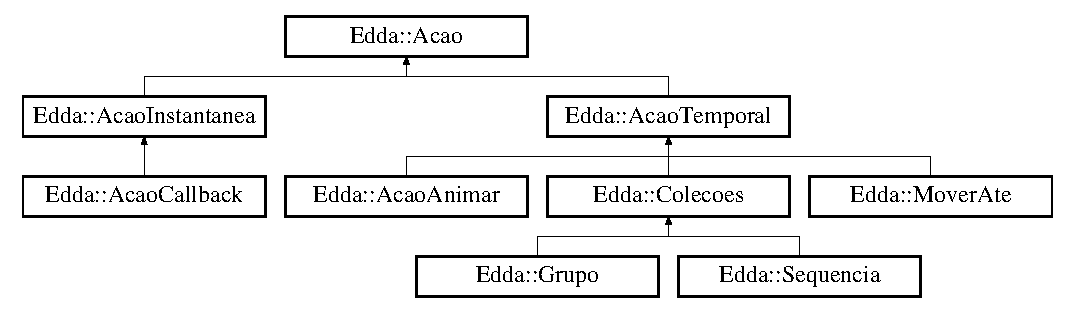
\includegraphics[height=3.758389cm]{class_edda_1_1_acao}
\end{center}
\end{figure}
\subsection*{Public Member Functions}
\begin{DoxyCompactItemize}
\item 
\hypertarget{class_edda_1_1_acao_a65b7e5dd79178b1474b202a3c34bb340}{
\hyperlink{class_edda_1_1_acao_a65b7e5dd79178b1474b202a3c34bb340}{Acao} ()}
\label{class_edda_1_1_acao_a65b7e5dd79178b1474b202a3c34bb340}

\begin{DoxyCompactList}\small\item\em Construtor padr�o da a��o \item\end{DoxyCompactList}\item 
\hypertarget{class_edda_1_1_acao_a372da0e8437dc11d02d26965ee1a2c0e}{
bool {\bfseries estaPronta} ()}
\label{class_edda_1_1_acao_a372da0e8437dc11d02d26965ee1a2c0e}

\item 
\hypertarget{class_edda_1_1_acao_a574b6e99fed8c960b62db8c375dfce1f}{
void {\bfseries parar} ()}
\label{class_edda_1_1_acao_a574b6e99fed8c960b62db8c375dfce1f}

\item 
\hypertarget{class_edda_1_1_acao_a31087d435bac96dde1b6f8cd7a7057f9}{
virtual void {\bfseries executar} (\hyperlink{class_edda_1_1_nodo}{Nodo} $\ast$)}
\label{class_edda_1_1_acao_a31087d435bac96dde1b6f8cd7a7057f9}

\item 
\hypertarget{class_edda_1_1_acao_a40ba1c27d975f7837742a72c942f0962}{
virtual void {\bfseries passo} (long dt)}
\label{class_edda_1_1_acao_a40ba1c27d975f7837742a72c942f0962}

\item 
\hypertarget{class_edda_1_1_acao_ae79993cbcda669283f77f36135a4a0a0}{
virtual void {\bfseries atualizar} (long)=0}
\label{class_edda_1_1_acao_ae79993cbcda669283f77f36135a4a0a0}

\end{DoxyCompactItemize}
\subsection*{Public Attributes}
\begin{DoxyCompactItemize}
\item 
int \hyperlink{class_edda_1_1_acao_a999ae2cf4c4b82ebdff8589e42f279a9}{tag}
\end{DoxyCompactItemize}
\subsection*{Protected Attributes}
\begin{DoxyCompactItemize}
\item 
\hyperlink{class_edda_1_1_nodo}{Nodo} $\ast$ \hyperlink{class_edda_1_1_acao_aae0c17808ed85e682bcc14f1a4065057}{alvo}
\item 
bool \hyperlink{class_edda_1_1_acao_a1f7eb7a2096978d8b66f31b8561e529a}{rodando}
\end{DoxyCompactItemize}


\subsection{Detailed Description}
Classe que descreve uma a��o Uma a��o modifica o estado de um nodo no tempo 

\subsection{Member Data Documentation}
\hypertarget{class_edda_1_1_acao_aae0c17808ed85e682bcc14f1a4065057}{
\index{Edda::Acao@{Edda::Acao}!alvo@{alvo}}
\index{alvo@{alvo}!Edda::Acao@{Edda::Acao}}
\subsubsection[{alvo}]{\setlength{\rightskip}{0pt plus 5cm}{\bf Nodo}$\ast$ {\bf Edda::Acao::alvo}\hspace{0.3cm}{\ttfamily  \mbox{[}protected\mbox{]}}}}
\label{class_edda_1_1_acao_aae0c17808ed85e682bcc14f1a4065057}
nodo alvo da a��o \hypertarget{class_edda_1_1_acao_a1f7eb7a2096978d8b66f31b8561e529a}{
\index{Edda::Acao@{Edda::Acao}!rodando@{rodando}}
\index{rodando@{rodando}!Edda::Acao@{Edda::Acao}}
\subsubsection[{rodando}]{\setlength{\rightskip}{0pt plus 5cm}bool {\bf Edda::Acao::rodando}\hspace{0.3cm}{\ttfamily  \mbox{[}protected\mbox{]}}}}
\label{class_edda_1_1_acao_a1f7eb7a2096978d8b66f31b8561e529a}
se a��o est� executando \hypertarget{class_edda_1_1_acao_a999ae2cf4c4b82ebdff8589e42f279a9}{
\index{Edda::Acao@{Edda::Acao}!tag@{tag}}
\index{tag@{tag}!Edda::Acao@{Edda::Acao}}
\subsubsection[{tag}]{\setlength{\rightskip}{0pt plus 5cm}int {\bf Edda::Acao::tag}}}
\label{class_edda_1_1_acao_a999ae2cf4c4b82ebdff8589e42f279a9}
id identifcador da a��o 

The documentation for this class was generated from the following files:\begin{DoxyCompactItemize}
\item 
Acao.h\item 
Acao.cpp\end{DoxyCompactItemize}

\hypertarget{class_edda_1_1_acao_animar}{
\section{Edda::AcaoAnimar Class Reference}
\label{class_edda_1_1_acao_animar}\index{Edda::AcaoAnimar@{Edda::AcaoAnimar}}
}
Inheritance diagram for Edda::AcaoAnimar:\begin{figure}[H]
\begin{center}
\leavevmode
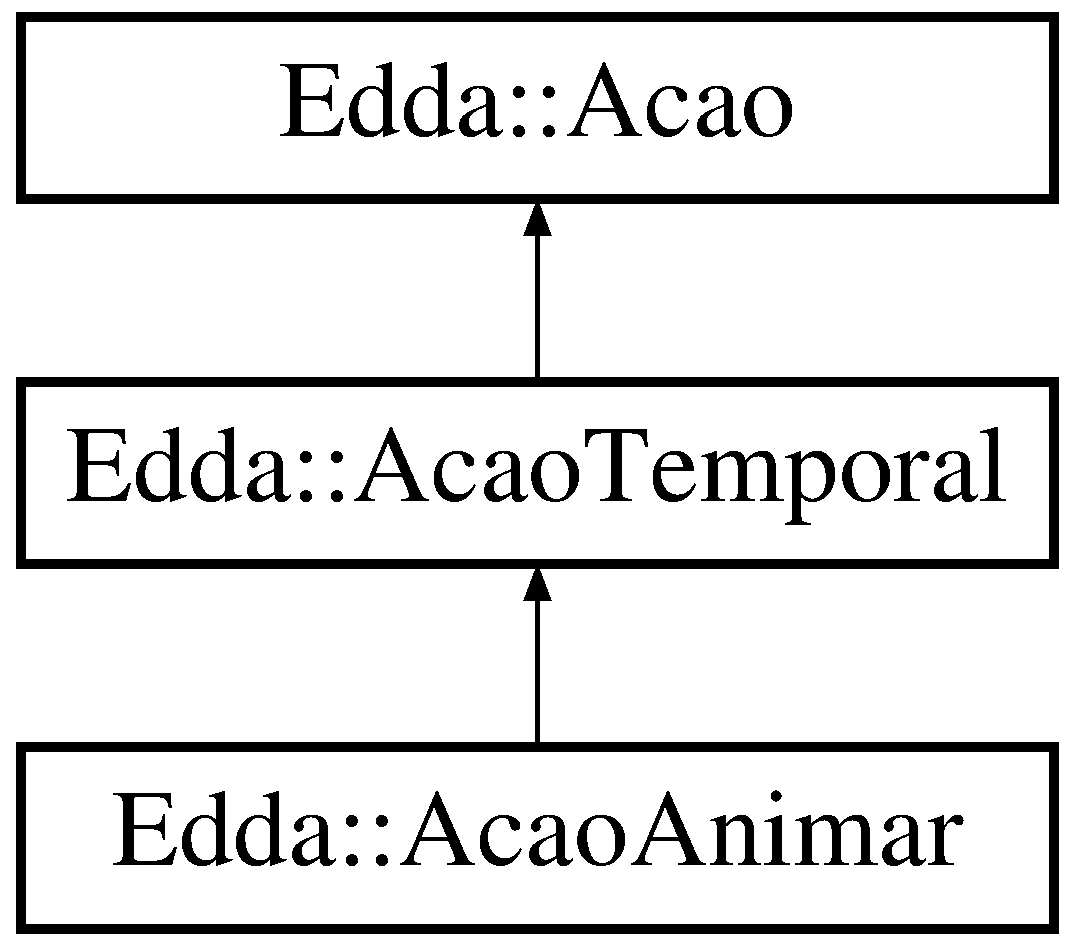
\includegraphics[height=3.000000cm]{class_edda_1_1_acao_animar}
\end{center}
\end{figure}
\subsection*{Public Member Functions}
\begin{DoxyCompactItemize}
\item 
\hypertarget{class_edda_1_1_acao_animar_a371c98cb4871124349c8b6be1c5a347c}{
{\bfseries AcaoAnimar} (\hyperlink{class_edda_1_1_animacao}{Animacao} $\ast$)}
\label{class_edda_1_1_acao_animar_a371c98cb4871124349c8b6be1c5a347c}

\item 
\hypertarget{class_edda_1_1_acao_animar_a22024ff76d5b145bb4f0497b0f91fcf8}{
void {\bfseries passo} (long)}
\label{class_edda_1_1_acao_animar_a22024ff76d5b145bb4f0497b0f91fcf8}

\item 
\hypertarget{class_edda_1_1_acao_animar_a05b8c14a5d9dd36ca2ddf129e529cfcb}{
void {\bfseries executar} (\hyperlink{class_edda_1_1_nodo}{Nodo} $\ast$)}
\label{class_edda_1_1_acao_animar_a05b8c14a5d9dd36ca2ddf129e529cfcb}

\end{DoxyCompactItemize}


The documentation for this class was generated from the following files:\begin{DoxyCompactItemize}
\item 
AcaoAnimar.h\item 
AcaoAnimar.cpp\end{DoxyCompactItemize}

\hypertarget{class_edda_1_1_acao_callback}{
\section{Edda::AcaoCallback Class Reference}
\label{class_edda_1_1_acao_callback}\index{Edda::AcaoCallback@{Edda::AcaoCallback}}
}
Inheritance diagram for Edda::AcaoCallback:\begin{figure}[H]
\begin{center}
\leavevmode
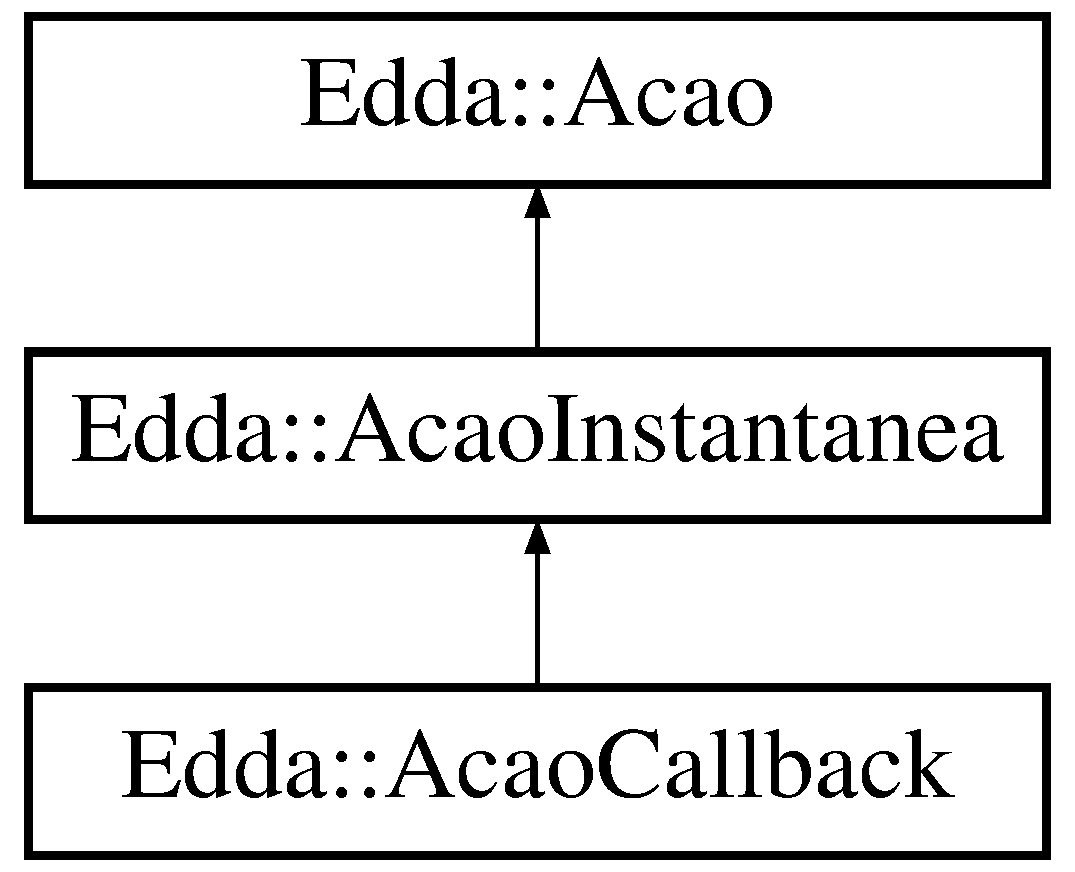
\includegraphics[height=3.000000cm]{class_edda_1_1_acao_callback}
\end{center}
\end{figure}
\subsection*{Public Member Functions}
\begin{DoxyCompactItemize}
\item 
\hypertarget{class_edda_1_1_acao_callback_aeeab21390d435dce7b293167280dfc32}{
{\bfseries AcaoCallback} (\hyperlink{class_edda_1_1_acao_listener}{AcaoListener} $\ast$, void $\ast$)}
\label{class_edda_1_1_acao_callback_aeeab21390d435dce7b293167280dfc32}

\item 
\hypertarget{class_edda_1_1_acao_callback_a87d22c6b8521ce1dadf4bb1d827b5204}{
void {\bfseries passo} (long)}
\label{class_edda_1_1_acao_callback_a87d22c6b8521ce1dadf4bb1d827b5204}

\end{DoxyCompactItemize}


The documentation for this class was generated from the following files:\begin{DoxyCompactItemize}
\item 
AcaoCallback.h\item 
AcaoCallback.cpp\end{DoxyCompactItemize}

\hypertarget{class_edda_1_1_acao_instantanea}{
\section{Edda::AcaoInstantanea Class Reference}
\label{class_edda_1_1_acao_instantanea}\index{Edda::AcaoInstantanea@{Edda::AcaoInstantanea}}
}
Inheritance diagram for Edda::AcaoInstantanea:\begin{figure}[H]
\begin{center}
\leavevmode
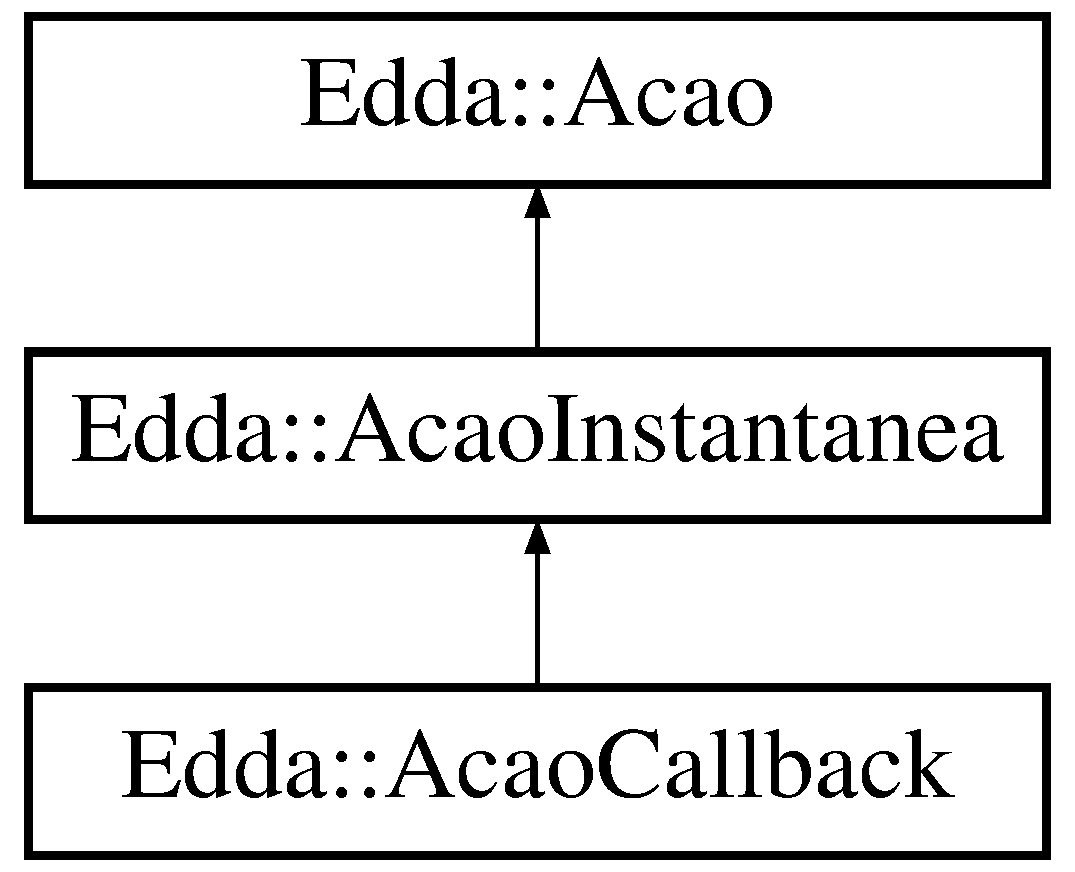
\includegraphics[height=3.000000cm]{class_edda_1_1_acao_instantanea}
\end{center}
\end{figure}
\subsection*{Public Member Functions}
\begin{DoxyCompactItemize}
\item 
\hypertarget{class_edda_1_1_acao_instantanea_ab00831705f1b6c385b07e15398ac8243}{
void {\bfseries atualizar} (long)}
\label{class_edda_1_1_acao_instantanea_ab00831705f1b6c385b07e15398ac8243}

\item 
\hypertarget{class_edda_1_1_acao_instantanea_a8847ea6960937282148d44d39ccc9e4f}{
long {\bfseries getDuracao} ()}
\label{class_edda_1_1_acao_instantanea_a8847ea6960937282148d44d39ccc9e4f}

\end{DoxyCompactItemize}


The documentation for this class was generated from the following files:\begin{DoxyCompactItemize}
\item 
AcaoInstantanea.h\item 
AcaoInstantanea.cpp\end{DoxyCompactItemize}

\hypertarget{class_edda_1_1_acao_listener}{
\section{Edda::AcaoListener Class Reference}
\label{class_edda_1_1_acao_listener}\index{Edda::AcaoListener@{Edda::AcaoListener}}
}
\subsection*{Public Member Functions}
\begin{DoxyCompactItemize}
\item 
\hypertarget{class_edda_1_1_acao_listener_ad77d35a56da6eafcb3597713594dad23}{
virtual void {\bfseries executar} (\hyperlink{class_edda_1_1_nodo}{Nodo} $\ast$, void $\ast$, long t)=0}
\label{class_edda_1_1_acao_listener_ad77d35a56da6eafcb3597713594dad23}

\end{DoxyCompactItemize}


The documentation for this class was generated from the following file:\begin{DoxyCompactItemize}
\item 
AcaoCallback.h\end{DoxyCompactItemize}

\hypertarget{class_edda_1_1_acao_temporal}{
\section{Edda::AcaoTemporal Class Reference}
\label{class_edda_1_1_acao_temporal}\index{Edda::AcaoTemporal@{Edda::AcaoTemporal}}
}
Inheritance diagram for Edda::AcaoTemporal:\begin{figure}[H]
\begin{center}
\leavevmode
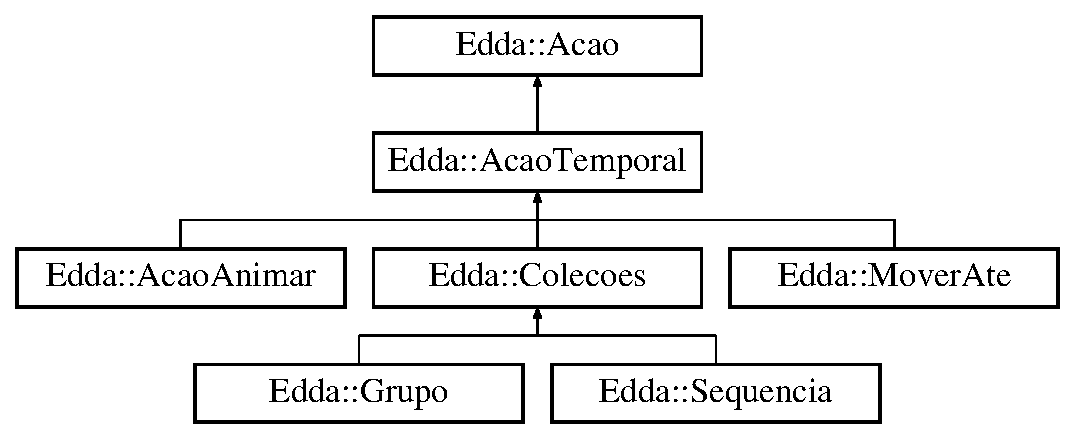
\includegraphics[height=4.000000cm]{class_edda_1_1_acao_temporal}
\end{center}
\end{figure}
\subsection*{Public Member Functions}
\begin{DoxyCompactItemize}
\item 
\hypertarget{class_edda_1_1_acao_temporal_a585f57574847220cb3ce909811084dbb}{
{\bfseries AcaoTemporal} (long d)}
\label{class_edda_1_1_acao_temporal_a585f57574847220cb3ce909811084dbb}

\item 
\hypertarget{class_edda_1_1_acao_temporal_a2ecc59bbbda5a2014c62320265a5a66a}{
void {\bfseries atualizar} (long)}
\label{class_edda_1_1_acao_temporal_a2ecc59bbbda5a2014c62320265a5a66a}

\item 
\hypertarget{class_edda_1_1_acao_temporal_a3406ed807ec09444176c9b7787cf3d81}{
long {\bfseries getDuracao} ()}
\label{class_edda_1_1_acao_temporal_a3406ed807ec09444176c9b7787cf3d81}

\end{DoxyCompactItemize}
\subsection*{Protected Attributes}
\begin{DoxyCompactItemize}
\item 
\hypertarget{class_edda_1_1_acao_temporal_a45d2f8a606fa0df86183476df84cc5f3}{
long {\bfseries duracao}}
\label{class_edda_1_1_acao_temporal_a45d2f8a606fa0df86183476df84cc5f3}

\end{DoxyCompactItemize}


The documentation for this class was generated from the following files:\begin{DoxyCompactItemize}
\item 
AcaoTemporal.h\item 
AcaoTemporal.cpp\end{DoxyCompactItemize}

\hypertarget{class_edda_1_1_animacao}{
\section{Edda::Animacao Class Reference}
\label{class_edda_1_1_animacao}\index{Edda::Animacao@{Edda::Animacao}}
}
\subsection*{Public Member Functions}
\begin{DoxyCompactItemize}
\item 
\hypertarget{class_edda_1_1_animacao_a8e93855aa667f7d249a41dcdc9ee8762}{
long {\bfseries getDuracao} ()}
\label{class_edda_1_1_animacao_a8e93855aa667f7d249a41dcdc9ee8762}

\item 
\hypertarget{class_edda_1_1_animacao_a60df33cc7ca86e9b2718632bd09fb2e0}{
int {\bfseries getTotalUnidades} ()}
\label{class_edda_1_1_animacao_a60df33cc7ca86e9b2718632bd09fb2e0}

\item 
\hypertarget{class_edda_1_1_animacao_adaca55e71720c0d1f98b9e4ef4a92bf0}{
long {\bfseries getDelay} (int)}
\label{class_edda_1_1_animacao_adaca55e71720c0d1f98b9e4ef4a92bf0}

\item 
\hypertarget{class_edda_1_1_animacao_a7714c3bd40eb8dc29ee7ab940bcf8f28}{
void {\bfseries adicionarFrame} (\hyperlink{class_edda_1_1_frame}{Frame} $\ast$)}
\label{class_edda_1_1_animacao_a7714c3bd40eb8dc29ee7ab940bcf8f28}

\item 
\hypertarget{class_edda_1_1_animacao_a64577e0a5b52359bc3881f8e84de0f7e}{
void {\bfseries adicionarFrames} (int $\ast$, int)}
\label{class_edda_1_1_animacao_a64577e0a5b52359bc3881f8e84de0f7e}

\item 
\hypertarget{class_edda_1_1_animacao_a77a1235c16fd5988bfd81d5fdd211f6f}{
void {\bfseries adicionarFrames} (int $\ast$, int $\ast$, int)}
\label{class_edda_1_1_animacao_a77a1235c16fd5988bfd81d5fdd211f6f}

\item 
\hypertarget{class_edda_1_1_animacao_a4a8dbfd437d9e76ee09399bc4ec0584d}{
void {\bfseries adicionarFrames} (int, int)}
\label{class_edda_1_1_animacao_a4a8dbfd437d9e76ee09399bc4ec0584d}

\end{DoxyCompactItemize}
\subsection*{Public Attributes}
\begin{DoxyCompactItemize}
\item 
\hypertarget{class_edda_1_1_animacao_af9f53cfbff194c5e23aa7a811e575ec2}{
int {\bfseries loops}}
\label{class_edda_1_1_animacao_af9f53cfbff194c5e23aa7a811e575ec2}

\item 
\hypertarget{class_edda_1_1_animacao_afba08a7be39e61375ec196d013809924}{
vector$<$ \hyperlink{class_edda_1_1_frame}{Frame} $\ast$ $>$ {\bfseries frames}}
\label{class_edda_1_1_animacao_afba08a7be39e61375ec196d013809924}

\item 
\hypertarget{class_edda_1_1_animacao_a92d56c89029f189ae78138b8d9c76653}{
\hyperlink{class_edda_1_1_sprite}{Sprite} $\ast$ {\bfseries sprite}}
\label{class_edda_1_1_animacao_a92d56c89029f189ae78138b8d9c76653}

\end{DoxyCompactItemize}


The documentation for this class was generated from the following files:\begin{DoxyCompactItemize}
\item 
Animacao.h\item 
Animacao.cpp\end{DoxyCompactItemize}

\hypertarget{class_edda_1_1_atualizavel}{
\section{Edda::Atualizavel Class Reference}
\label{class_edda_1_1_atualizavel}\index{Edda::Atualizavel@{Edda::Atualizavel}}
}
\subsection*{Public Member Functions}
\begin{DoxyCompactItemize}
\item 
\hypertarget{class_edda_1_1_atualizavel_a5b8c6f41e2fd8d47612d0b949efe2b14}{
virtual void {\bfseries atualizar} (long)=0}
\label{class_edda_1_1_atualizavel_a5b8c6f41e2fd8d47612d0b949efe2b14}

\end{DoxyCompactItemize}


The documentation for this class was generated from the following file:\begin{DoxyCompactItemize}
\item 
Diretor.h\end{DoxyCompactItemize}

\hypertarget{class_edda_1_1_camada}{
\section{Edda::Camada Class Reference}
\label{class_edda_1_1_camada}\index{Edda::Camada@{Edda::Camada}}
}
Inheritance diagram for Edda::Camada:\begin{figure}[H]
\begin{center}
\leavevmode
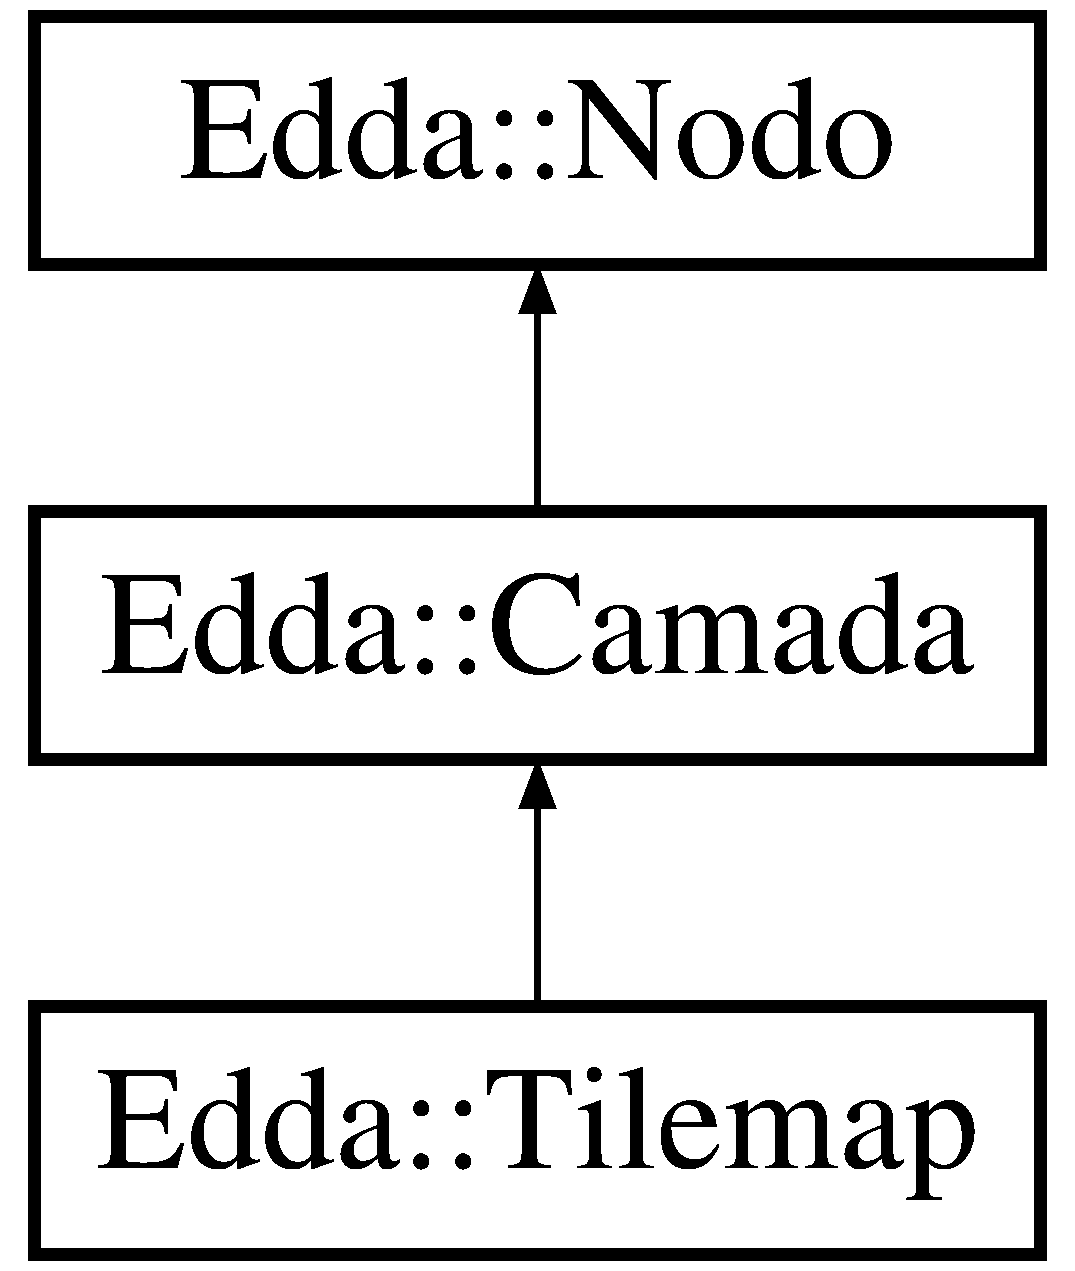
\includegraphics[height=3.000000cm]{class_edda_1_1_camada}
\end{center}
\end{figure}
\subsection*{Public Member Functions}
\begin{DoxyCompactItemize}
\item 
\hypertarget{class_edda_1_1_camada_a9ca2592c914f8a071604a20f7088818b}{
{\bfseries Camada} (int, int, int, int a=0)}
\label{class_edda_1_1_camada_a9ca2592c914f8a071604a20f7088818b}

\item 
\hypertarget{class_edda_1_1_camada_afac6eae74e2af943636e3ff93c2fb2d7}{
void {\bfseries desenhar} (RenderWindow $\ast$)}
\label{class_edda_1_1_camada_afac6eae74e2af943636e3ff93c2fb2d7}

\item 
\hypertarget{class_edda_1_1_camada_a33c1914ece04b8fc16c1762c932e99c4}{
void {\bfseries adicionar} (\hyperlink{class_edda_1_1_nodo}{Nodo} $\ast$n)}
\label{class_edda_1_1_camada_a33c1914ece04b8fc16c1762c932e99c4}

\item 
\hypertarget{class_edda_1_1_camada_a6ba56fdf8a66e08ef7e20aaaf43e4fba}{
void {\bfseries remover} (\hyperlink{class_edda_1_1_nodo}{Nodo} $\ast$n)}
\label{class_edda_1_1_camada_a6ba56fdf8a66e08ef7e20aaaf43e4fba}

\item 
\hypertarget{class_edda_1_1_camada_a79606763972bb5760d8d3e7537652220}{
void {\bfseries tratarEvento} (RenderWindow $\ast$)}
\label{class_edda_1_1_camada_a79606763972bb5760d8d3e7537652220}

\end{DoxyCompactItemize}
\subsection*{Protected Attributes}
\begin{DoxyCompactItemize}
\item 
\hypertarget{class_edda_1_1_camada_a77cba40ab2d88d80ed2b4bc8e071799e}{
list$<$ \hyperlink{class_edda_1_1_nodo}{Nodo} $\ast$ $>$ {\bfseries nodos}}
\label{class_edda_1_1_camada_a77cba40ab2d88d80ed2b4bc8e071799e}

\end{DoxyCompactItemize}


The documentation for this class was generated from the following files:\begin{DoxyCompactItemize}
\item 
Camada.h\item 
Camada.cpp\end{DoxyCompactItemize}

\hypertarget{class_edda_1_1_cena}{
\section{Edda::Cena Class Reference}
\label{class_edda_1_1_cena}\index{Edda::Cena@{Edda::Cena}}
}
Inheritance diagram for Edda::Cena:\begin{figure}[H]
\begin{center}
\leavevmode
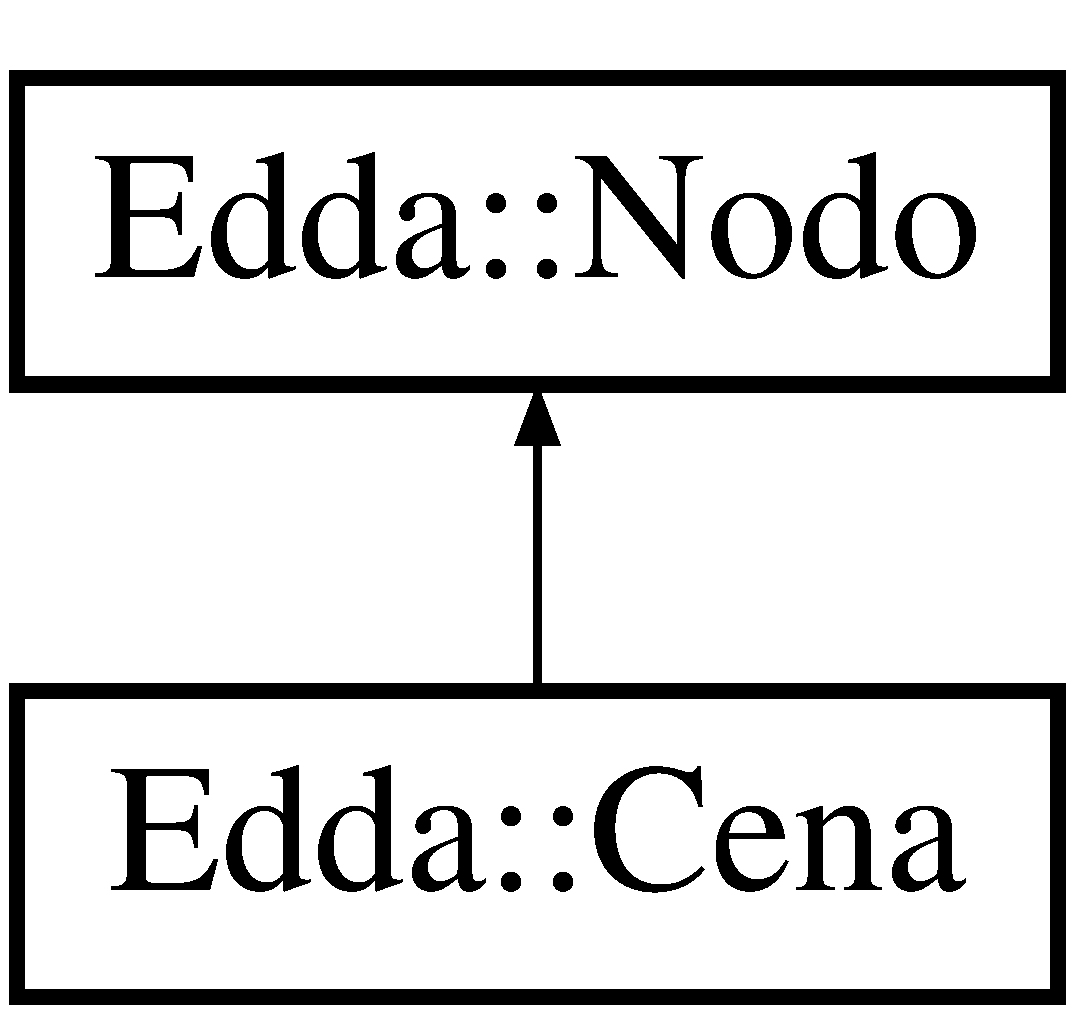
\includegraphics[height=2.000000cm]{class_edda_1_1_cena}
\end{center}
\end{figure}
\subsection*{Public Member Functions}
\begin{DoxyCompactItemize}
\item 
\hypertarget{class_edda_1_1_cena_aadddd43658f20231e2a4791c2c321c36}{
void {\bfseries desenhar} (RenderWindow $\ast$)}
\label{class_edda_1_1_cena_aadddd43658f20231e2a4791c2c321c36}

\item 
\hypertarget{class_edda_1_1_cena_a9b5584b195340f2992d2beea4cd36ca7}{
void {\bfseries tratarEvento} (RenderWindow $\ast$)}
\label{class_edda_1_1_cena_a9b5584b195340f2992d2beea4cd36ca7}

\end{DoxyCompactItemize}


The documentation for this class was generated from the following files:\begin{DoxyCompactItemize}
\item 
Cena.h\item 
Cena.cpp\end{DoxyCompactItemize}

\hypertarget{class_edda_1_1_colecoes}{
\section{Edda::Colecoes Class Reference}
\label{class_edda_1_1_colecoes}\index{Edda::Colecoes@{Edda::Colecoes}}
}
Inheritance diagram for Edda::Colecoes:\begin{figure}[H]
\begin{center}
\leavevmode
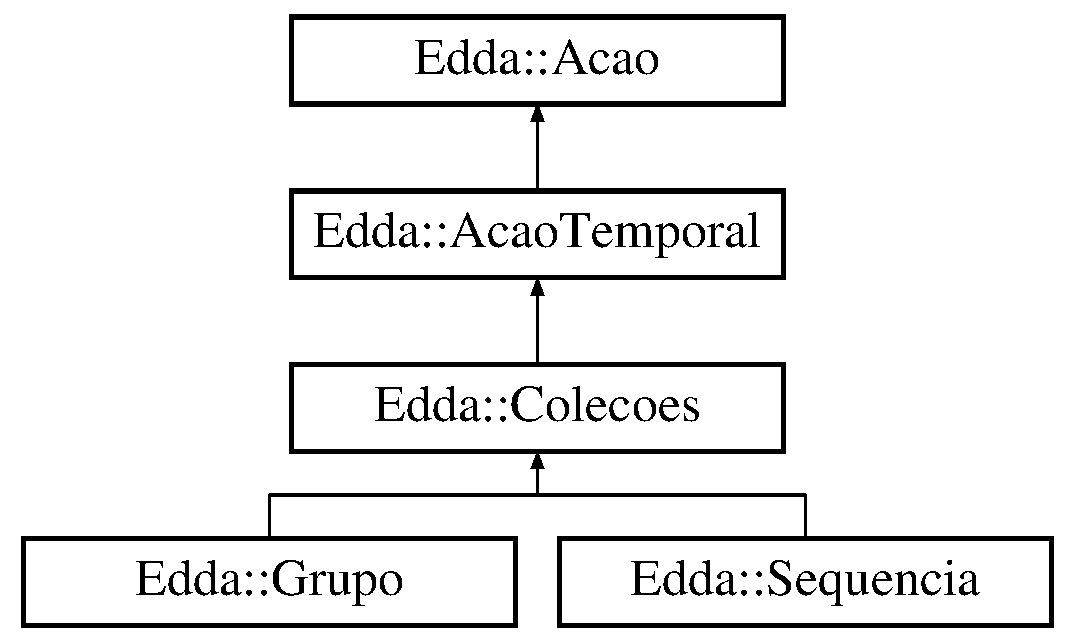
\includegraphics[height=4.000000cm]{class_edda_1_1_colecoes}
\end{center}
\end{figure}
\subsection*{Public Member Functions}
\begin{DoxyCompactItemize}
\item 
\hypertarget{class_edda_1_1_colecoes_a0d96c9eec71a2aba4c97e6643bbdd727}{
void {\bfseries adicionar} (\hyperlink{class_edda_1_1_acao_temporal}{AcaoTemporal} $\ast$)}
\label{class_edda_1_1_colecoes_a0d96c9eec71a2aba4c97e6643bbdd727}

\item 
\hypertarget{class_edda_1_1_colecoes_a16264ec49b8b56cb3836460bb67ad919}{
void {\bfseries executar} (\hyperlink{class_edda_1_1_nodo}{Nodo} $\ast$n)}
\label{class_edda_1_1_colecoes_a16264ec49b8b56cb3836460bb67ad919}

\item 
\hypertarget{class_edda_1_1_colecoes_a837da11bffd93be4860a68a2b297db92}{
void {\bfseries passo} (long)}
\label{class_edda_1_1_colecoes_a837da11bffd93be4860a68a2b297db92}

\end{DoxyCompactItemize}
\subsection*{Protected Attributes}
\begin{DoxyCompactItemize}
\item 
\hypertarget{class_edda_1_1_colecoes_a678033cea1724264a53b0c088f03c0f2}{
vector$<$ \hyperlink{class_edda_1_1_acao_temporal}{AcaoTemporal} $\ast$ $>$ {\bfseries acoes}}
\label{class_edda_1_1_colecoes_a678033cea1724264a53b0c088f03c0f2}

\item 
\hypertarget{class_edda_1_1_colecoes_a2544748c74e6d17195ed57f85d70666f}{
int {\bfseries pos}}
\label{class_edda_1_1_colecoes_a2544748c74e6d17195ed57f85d70666f}

\end{DoxyCompactItemize}


The documentation for this class was generated from the following files:\begin{DoxyCompactItemize}
\item 
Colecoes.h\item 
Colecoes.cpp\end{DoxyCompactItemize}

\hypertarget{class_collision}{
\section{Collision Class Reference}
\label{class_collision}\index{Collision@{Collision}}
}
\subsection*{Static Public Member Functions}
\begin{DoxyCompactItemize}
\item 
static bool \hyperlink{class_collision_ae2fac0fb78ba69f8fe0301dedce492be}{PixelPerfectTest} (const sf::Sprite \&Object1, const sf::Sprite \&Object2, sf::Uint8 AlphaLimit=127)
\item 
static bool \hyperlink{class_collision_af2f8835beee81b76d04311c794c36c0f}{CircleTest} (const sf::Sprite \&Object1, const sf::Sprite \&Object2)
\item 
static bool \hyperlink{class_collision_a6f5945d467e629017010b139062919c6}{BoundingBoxTest} (const sf::Sprite \&Object1, const sf::Sprite \&Object2)
\item 
static sf::IntRect \hyperlink{class_collision_afacb4e2c95010ac68c560f437be251aa}{GetAABB} (const sf::Sprite \&Object)
\item 
static sf::Vector2f \hyperlink{class_collision_aba800d3b1e206e05fd787d025d41bae9}{RotatePoint} (const sf::Vector2f \&Point, float Angle)
\item 
static float \hyperlink{class_collision_aeef6bf21c0f1ebf170df04c1957da0ad}{MinValue} (float a, float b, float c, float d)
\item 
static float \hyperlink{class_collision_ab2395ef5aa96a4030d74adbfe5d624fe}{MaxValue} (float a, float b, float c, float d)
\end{DoxyCompactItemize}


\subsection{Member Function Documentation}
\hypertarget{class_collision_a6f5945d467e629017010b139062919c6}{
\index{Collision@{Collision}!BoundingBoxTest@{BoundingBoxTest}}
\index{BoundingBoxTest@{BoundingBoxTest}!Collision@{Collision}}
\subsubsection[{BoundingBoxTest}]{\setlength{\rightskip}{0pt plus 5cm}bool Collision::BoundingBoxTest (
\begin{DoxyParamCaption}
\item[{const sf::Sprite \&}]{ Object1, }
\item[{const sf::Sprite \&}]{ Object2}
\end{DoxyParamCaption}
)\hspace{0.3cm}{\ttfamily  \mbox{[}static\mbox{]}}}}
\label{class_collision_a6f5945d467e629017010b139062919c6}
Test for bounding box collision using OBB Box. To test against AABB use PixelPerfectTest with AlphaLimit = 0

\begin{DoxySeeAlso}{See also}
\hyperlink{class_collision_ae2fac0fb78ba69f8fe0301dedce492be}{Collision::PixelPerfectTest} 
\end{DoxySeeAlso}
\hypertarget{class_collision_af2f8835beee81b76d04311c794c36c0f}{
\index{Collision@{Collision}!CircleTest@{CircleTest}}
\index{CircleTest@{CircleTest}!Collision@{Collision}}
\subsubsection[{CircleTest}]{\setlength{\rightskip}{0pt plus 5cm}bool Collision::CircleTest (
\begin{DoxyParamCaption}
\item[{const sf::Sprite \&}]{ Object1, }
\item[{const sf::Sprite \&}]{ Object2}
\end{DoxyParamCaption}
)\hspace{0.3cm}{\ttfamily  \mbox{[}static\mbox{]}}}}
\label{class_collision_af2f8835beee81b76d04311c794c36c0f}
Test for collision using circle collision dection Radius is averaged from the dimesnions of the sprite so roughly circular objects will be much more accurate \hypertarget{class_collision_afacb4e2c95010ac68c560f437be251aa}{
\index{Collision@{Collision}!GetAABB@{GetAABB}}
\index{GetAABB@{GetAABB}!Collision@{Collision}}
\subsubsection[{GetAABB}]{\setlength{\rightskip}{0pt plus 5cm}sf::IntRect Collision::GetAABB (
\begin{DoxyParamCaption}
\item[{const sf::Sprite \&}]{ Object}
\end{DoxyParamCaption}
)\hspace{0.3cm}{\ttfamily  \mbox{[}static\mbox{]}}}}
\label{class_collision_afacb4e2c95010ac68c560f437be251aa}
Generate a Axis-\/Aligned Bounding Box for broad phase of Pixel Perfect detection.

\begin{DoxyReturn}{Returns}
IntRect to round off Floating point positions. 
\end{DoxyReturn}
\hypertarget{class_collision_ab2395ef5aa96a4030d74adbfe5d624fe}{
\index{Collision@{Collision}!MaxValue@{MaxValue}}
\index{MaxValue@{MaxValue}!Collision@{Collision}}
\subsubsection[{MaxValue}]{\setlength{\rightskip}{0pt plus 5cm}float Collision::MaxValue (
\begin{DoxyParamCaption}
\item[{float}]{ a, }
\item[{float}]{ b, }
\item[{float}]{ c, }
\item[{float}]{ d}
\end{DoxyParamCaption}
)\hspace{0.3cm}{\ttfamily  \mbox{[}static\mbox{]}}}}
\label{class_collision_ab2395ef5aa96a4030d74adbfe5d624fe}
Helper function to get the maximum from a list of values \hypertarget{class_collision_aeef6bf21c0f1ebf170df04c1957da0ad}{
\index{Collision@{Collision}!MinValue@{MinValue}}
\index{MinValue@{MinValue}!Collision@{Collision}}
\subsubsection[{MinValue}]{\setlength{\rightskip}{0pt plus 5cm}float Collision::MinValue (
\begin{DoxyParamCaption}
\item[{float}]{ a, }
\item[{float}]{ b, }
\item[{float}]{ c, }
\item[{float}]{ d}
\end{DoxyParamCaption}
)\hspace{0.3cm}{\ttfamily  \mbox{[}static\mbox{]}}}}
\label{class_collision_aeef6bf21c0f1ebf170df04c1957da0ad}
Helper function to get the minimum from a list of values \hypertarget{class_collision_ae2fac0fb78ba69f8fe0301dedce492be}{
\index{Collision@{Collision}!PixelPerfectTest@{PixelPerfectTest}}
\index{PixelPerfectTest@{PixelPerfectTest}!Collision@{Collision}}
\subsubsection[{PixelPerfectTest}]{\setlength{\rightskip}{0pt plus 5cm}bool Collision::PixelPerfectTest (
\begin{DoxyParamCaption}
\item[{const sf::Sprite \&}]{ Object1, }
\item[{const sf::Sprite \&}]{ Object2, }
\item[{sf::Uint8}]{ AlphaLimit = {\ttfamily 127}}
\end{DoxyParamCaption}
)\hspace{0.3cm}{\ttfamily  \mbox{[}static\mbox{]}}}}
\label{class_collision_ae2fac0fb78ba69f8fe0301dedce492be}
Test for a pixel perfect collision detection between two Sprites, Rotation and Scale is supported in this test


\begin{DoxyParams}{Parameters}
{\em Object1} & The first sprite \\
\hline
{\em Object2} & The second sprite  How opaque a pixel needs to be before a hit it registered \\
\hline
\end{DoxyParams}
\hypertarget{class_collision_aba800d3b1e206e05fd787d025d41bae9}{
\index{Collision@{Collision}!RotatePoint@{RotatePoint}}
\index{RotatePoint@{RotatePoint}!Collision@{Collision}}
\subsubsection[{RotatePoint}]{\setlength{\rightskip}{0pt plus 5cm}sf::Vector2f Collision::RotatePoint (
\begin{DoxyParamCaption}
\item[{const sf::Vector2f \&}]{ Point, }
\item[{float}]{ Angle}
\end{DoxyParamCaption}
)\hspace{0.3cm}{\ttfamily  \mbox{[}static\mbox{]}}}}
\label{class_collision_aba800d3b1e206e05fd787d025d41bae9}
Helper function in order to rotate a point by an Angle

Rotation is CounterClockwise in order to match SFML Sprite Rotation


\begin{DoxyParams}{Parameters}
{\em Point} & a Vector2f representing a coordinate \\
\hline
{\em Angle} & angle in degrees \\
\hline
\end{DoxyParams}


The documentation for this class was generated from the following files:\begin{DoxyCompactItemize}
\item 
Collision.h\item 
Collision.cpp\end{DoxyCompactItemize}

\hypertarget{class_edda_1_1_cor}{
\section{Edda::Cor Class Reference}
\label{class_edda_1_1_cor}\index{Edda::Cor@{Edda::Cor}}
}
\subsection*{Public Attributes}
\begin{DoxyCompactItemize}
\item 
\hypertarget{class_edda_1_1_cor_a2797d86a904dfa765297c342de7b030f}{
int {\bfseries r}}
\label{class_edda_1_1_cor_a2797d86a904dfa765297c342de7b030f}

\item 
\hypertarget{class_edda_1_1_cor_a65c778444daee740522aa93eccbf776f}{
int {\bfseries g}}
\label{class_edda_1_1_cor_a65c778444daee740522aa93eccbf776f}

\item 
\hypertarget{class_edda_1_1_cor_a1483312898fc65da9c3c57b89c32fb91}{
int {\bfseries b}}
\label{class_edda_1_1_cor_a1483312898fc65da9c3c57b89c32fb91}

\item 
\hypertarget{class_edda_1_1_cor_a4fa3913e99eb13b7ed15e8b82106f8ff}{
int {\bfseries a}}
\label{class_edda_1_1_cor_a4fa3913e99eb13b7ed15e8b82106f8ff}

\end{DoxyCompactItemize}


The documentation for this class was generated from the following file:\begin{DoxyCompactItemize}
\item 
Cor.h\end{DoxyCompactItemize}

\hypertarget{class_edda_1_1_diretor}{
\section{Edda::Diretor Class Reference}
\label{class_edda_1_1_diretor}\index{Edda::Diretor@{Edda::Diretor}}
}
\subsection*{Public Member Functions}
\begin{DoxyCompactItemize}
\item 
\hypertarget{class_edda_1_1_diretor_afe1cdd2433db4a3fa28218b21e60cd2c}{
void {\bfseries iniciar} (int, int, int, string, bool fullscreen=false)}
\label{class_edda_1_1_diretor_afe1cdd2433db4a3fa28218b21e60cd2c}

\item 
\hypertarget{class_edda_1_1_diretor_af5b5db70fbf16b8a0faa8db3c5cb3e05}{
void {\bfseries adicionarCena} (\hyperlink{class_edda_1_1_cena}{Cena} $\ast$c)}
\label{class_edda_1_1_diretor_af5b5db70fbf16b8a0faa8db3c5cb3e05}

\item 
\hypertarget{class_edda_1_1_diretor_aee3297f8d86fc9ebb72492c0bfb1d4ef}{
void {\bfseries loop} (\hyperlink{class_edda_1_1_cena}{Cena} $\ast$c)}
\label{class_edda_1_1_diretor_aee3297f8d86fc9ebb72492c0bfb1d4ef}

\item 
\hypertarget{class_edda_1_1_diretor_a82a8443066bc07a5453a45ca7a07f914}{
void {\bfseries adicionarAtualizavel} (\hyperlink{class_edda_1_1_atualizavel}{Atualizavel} $\ast$)}
\label{class_edda_1_1_diretor_a82a8443066bc07a5453a45ca7a07f914}

\item 
\hypertarget{class_edda_1_1_diretor_a09e772049dd1e91490620035ef5b9e39}{
void {\bfseries limparAtualizaveis} ()}
\label{class_edda_1_1_diretor_a09e772049dd1e91490620035ef5b9e39}

\end{DoxyCompactItemize}
\subsection*{Static Public Member Functions}
\begin{DoxyCompactItemize}
\item 
\hypertarget{class_edda_1_1_diretor_a1da02fb61b36933484e242f581f17392}{
static \hyperlink{class_edda_1_1_diretor}{Diretor} $\ast$ {\bfseries getInstancia} ()}
\label{class_edda_1_1_diretor_a1da02fb61b36933484e242f581f17392}

\end{DoxyCompactItemize}
\subsection*{Public Attributes}
\begin{DoxyCompactItemize}
\item 
\hypertarget{class_edda_1_1_diretor_a8f8ddcb338b975fa7b8cfaa51511b119}{
int {\bfseries larguraTela}}
\label{class_edda_1_1_diretor_a8f8ddcb338b975fa7b8cfaa51511b119}

\item 
\hypertarget{class_edda_1_1_diretor_aeb88898002f2a81c6c0b2ac869720869}{
int {\bfseries alturaTela}}
\label{class_edda_1_1_diretor_aeb88898002f2a81c6c0b2ac869720869}

\end{DoxyCompactItemize}


The documentation for this class was generated from the following files:\begin{DoxyCompactItemize}
\item 
Diretor.h\item 
Diretor.cpp\end{DoxyCompactItemize}

\hypertarget{class_edda_1_1_frame}{
\section{Edda::Frame Class Reference}
\label{class_edda_1_1_frame}\index{Edda::Frame@{Edda::Frame}}
}
\subsection*{Public Member Functions}
\begin{DoxyCompactItemize}
\item 
\hypertarget{class_edda_1_1_frame_adc9957b371722fdb61270cf17a7651e8}{
{\bfseries Frame} (int i, long d=1)}
\label{class_edda_1_1_frame_adc9957b371722fdb61270cf17a7651e8}

\end{DoxyCompactItemize}
\subsection*{Public Attributes}
\begin{DoxyCompactItemize}
\item 
\hypertarget{class_edda_1_1_frame_ae64bf41c79f414270a7c686bafa23a79}{
int {\bfseries indexFrame}}
\label{class_edda_1_1_frame_ae64bf41c79f414270a7c686bafa23a79}

\item 
\hypertarget{class_edda_1_1_frame_ac28f41c0035b31f46bd29ee68006edc9}{
long {\bfseries unidadesDelay}}
\label{class_edda_1_1_frame_ac28f41c0035b31f46bd29ee68006edc9}

\end{DoxyCompactItemize}


The documentation for this class was generated from the following file:\begin{DoxyCompactItemize}
\item 
Animacao.h\end{DoxyCompactItemize}

\hypertarget{class_edda_1_1_grupo}{
\section{Edda::Grupo Class Reference}
\label{class_edda_1_1_grupo}\index{Edda::Grupo@{Edda::Grupo}}
}
Inheritance diagram for Edda::Grupo:\begin{figure}[H]
\begin{center}
\leavevmode
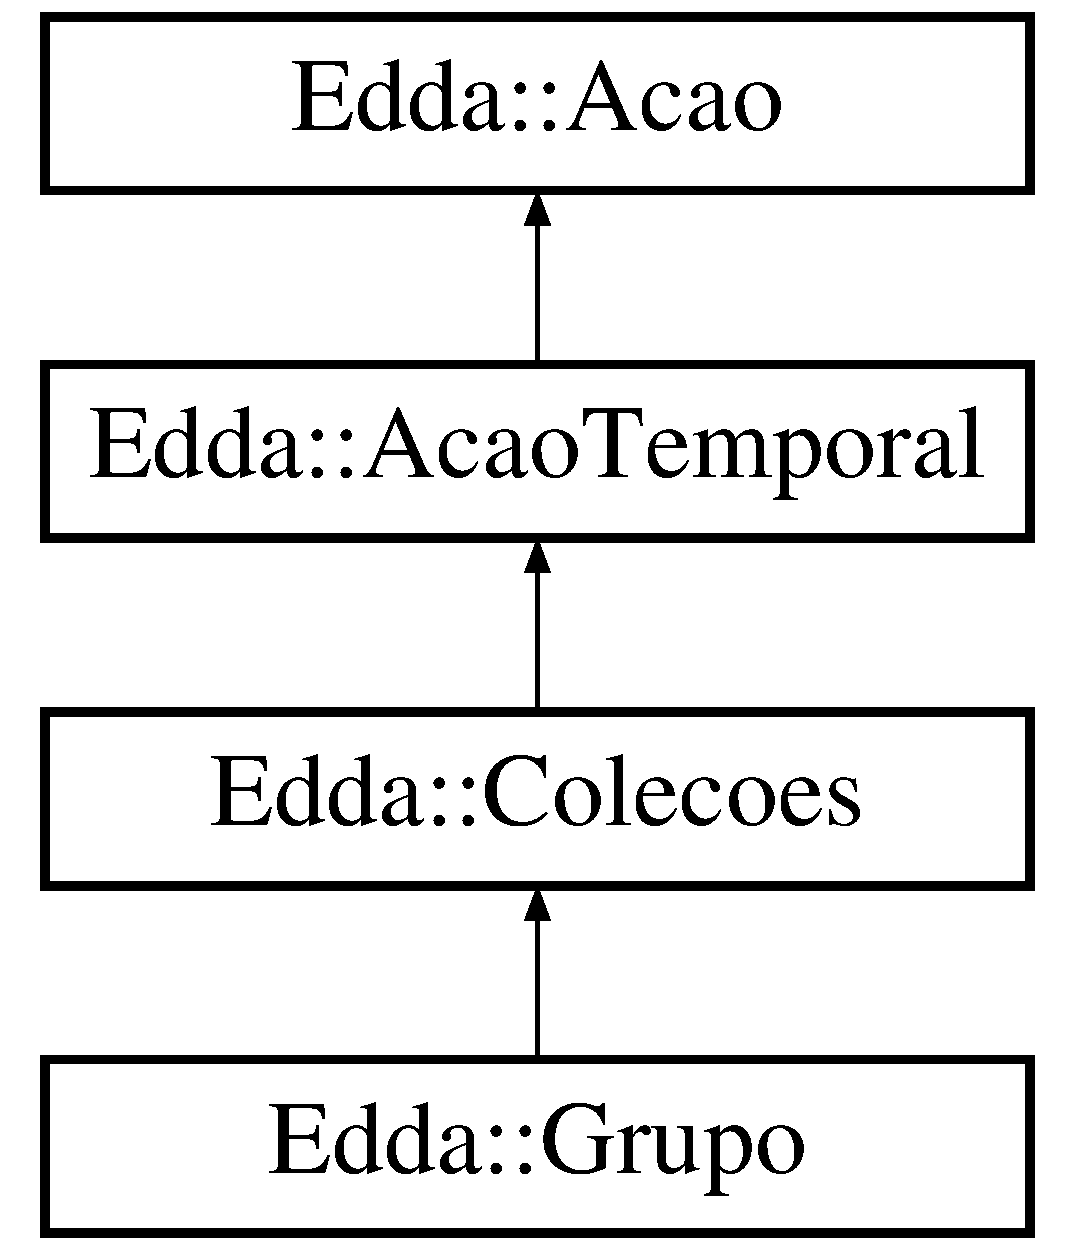
\includegraphics[height=4.000000cm]{class_edda_1_1_grupo}
\end{center}
\end{figure}
\subsection*{Public Member Functions}
\begin{DoxyCompactItemize}
\item 
\hypertarget{class_edda_1_1_grupo_abb4f5839bebf0dfd801f0e53e316a0a1}{
void {\bfseries atualizar} (long)}
\label{class_edda_1_1_grupo_abb4f5839bebf0dfd801f0e53e316a0a1}

\end{DoxyCompactItemize}


The documentation for this class was generated from the following files:\begin{DoxyCompactItemize}
\item 
Grupo.h\item 
Grupo.cpp\end{DoxyCompactItemize}

\hypertarget{class_edda_1_1_mover_ate}{
\section{Edda::MoverAte Class Reference}
\label{class_edda_1_1_mover_ate}\index{Edda::MoverAte@{Edda::MoverAte}}
}
Inheritance diagram for Edda::MoverAte:\begin{figure}[H]
\begin{center}
\leavevmode
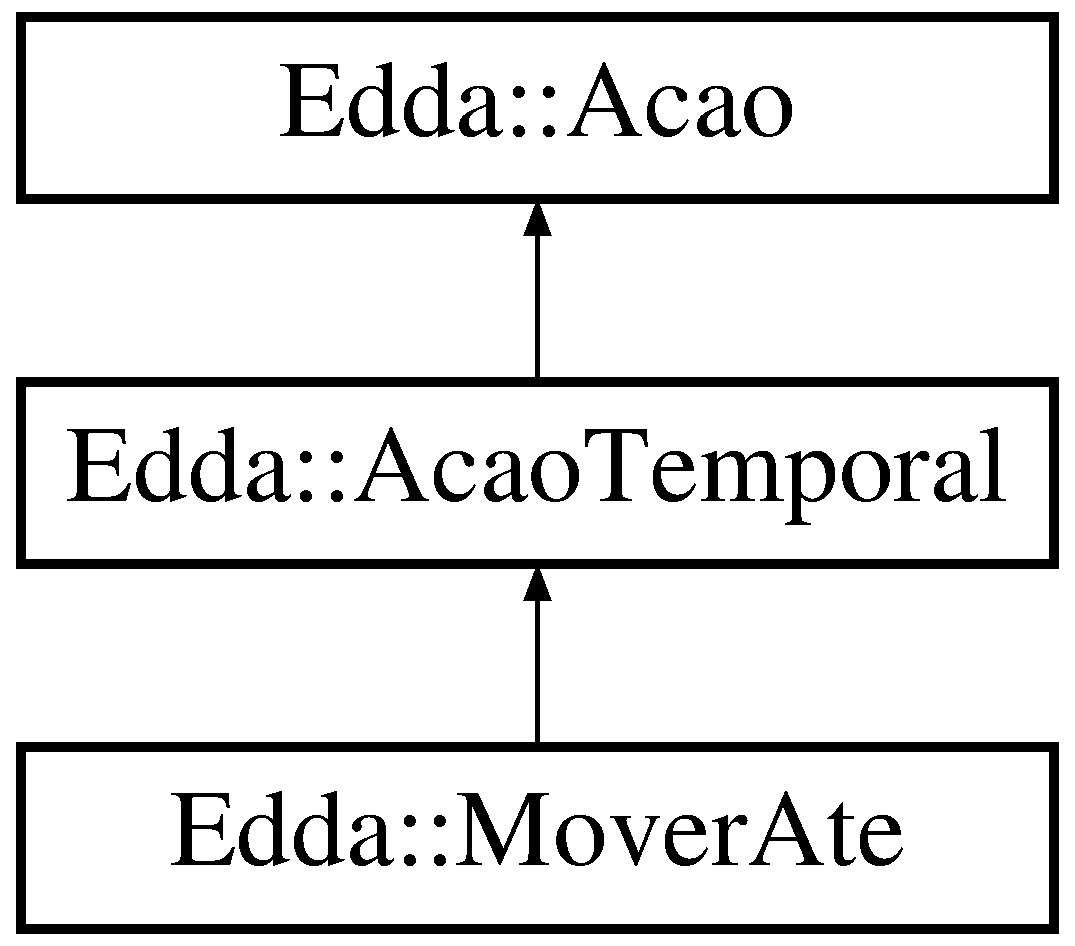
\includegraphics[height=3.000000cm]{class_edda_1_1_mover_ate}
\end{center}
\end{figure}
\subsection*{Public Member Functions}
\begin{DoxyCompactItemize}
\item 
\hypertarget{class_edda_1_1_mover_ate_ae6a0c17d19a4e150d2256fcc49b7e47a}{
{\bfseries MoverAte} (int x, int y, long d)}
\label{class_edda_1_1_mover_ate_ae6a0c17d19a4e150d2256fcc49b7e47a}

\item 
\hypertarget{class_edda_1_1_mover_ate_a4a3f80857082e611b614874e8f03b6f0}{
void {\bfseries passo} (long)}
\label{class_edda_1_1_mover_ate_a4a3f80857082e611b614874e8f03b6f0}

\item 
\hypertarget{class_edda_1_1_mover_ate_a911667d2bb87327c148fbbbe97e5a633}{
void {\bfseries executar} (\hyperlink{class_edda_1_1_nodo}{Nodo} $\ast$)}
\label{class_edda_1_1_mover_ate_a911667d2bb87327c148fbbbe97e5a633}

\end{DoxyCompactItemize}


The documentation for this class was generated from the following files:\begin{DoxyCompactItemize}
\item 
MoverAte.h\item 
MoverAte.cpp\end{DoxyCompactItemize}

\hypertarget{class_edda_1_1_nodo}{
\section{Edda::Nodo Class Reference}
\label{class_edda_1_1_nodo}\index{Edda::Nodo@{Edda::Nodo}}
}
Inheritance diagram for Edda::Nodo:\begin{figure}[H]
\begin{center}
\leavevmode
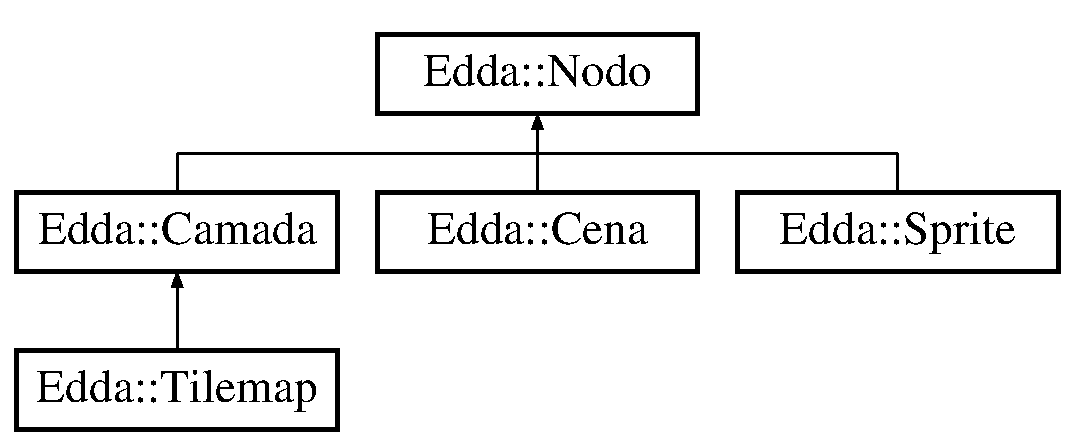
\includegraphics[height=3.000000cm]{class_edda_1_1_nodo}
\end{center}
\end{figure}
\subsection*{Public Member Functions}
\begin{DoxyCompactItemize}
\item 
\hypertarget{class_edda_1_1_nodo_aedc6c999c03cc00e41beddec7c93dac3}{
virtual void {\bfseries desenhar} (RenderWindow $\ast$)=0}
\label{class_edda_1_1_nodo_aedc6c999c03cc00e41beddec7c93dac3}

\item 
\hypertarget{class_edda_1_1_nodo_a0f24efb7a6f9be8e45b4ef2656c1e382}{
virtual void {\bfseries tratarEvento} (RenderWindow $\ast$)=0}
\label{class_edda_1_1_nodo_a0f24efb7a6f9be8e45b4ef2656c1e382}

\item 
\hypertarget{class_edda_1_1_nodo_a6c6ac09aa6ecb67c846ab6cb969d1c6d}{
void {\bfseries adicionar} (\hyperlink{class_edda_1_1_nodo}{Nodo} $\ast$n)}
\label{class_edda_1_1_nodo_a6c6ac09aa6ecb67c846ab6cb969d1c6d}

\item 
\hypertarget{class_edda_1_1_nodo_a9364a90f623ae04ba4752c1bef85ccdd}{
void {\bfseries remover} (\hyperlink{class_edda_1_1_nodo}{Nodo} $\ast$n)}
\label{class_edda_1_1_nodo_a9364a90f623ae04ba4752c1bef85ccdd}

\item 
\hypertarget{class_edda_1_1_nodo_a63d456d79bea395f8205261f364d7b90}{
\hyperlink{class_edda_1_1_nodo}{Nodo} $\ast$ {\bfseries pegarNodoPelaTag} (int tag)}
\label{class_edda_1_1_nodo_a63d456d79bea395f8205261f364d7b90}

\item 
\hypertarget{class_edda_1_1_nodo_a8b37a33842de487cabcefe72cd4dd483}{
void {\bfseries executar} ()}
\label{class_edda_1_1_nodo_a8b37a33842de487cabcefe72cd4dd483}

\item 
\hypertarget{class_edda_1_1_nodo_aecae42361dd3003dbae41b587161059b}{
void {\bfseries adicionarAcao} (\hyperlink{class_edda_1_1_acao}{Acao} $\ast$)}
\label{class_edda_1_1_nodo_aecae42361dd3003dbae41b587161059b}

\item 
\hypertarget{class_edda_1_1_nodo_a103bee6bcafc28294a1723423693cac4}{
void {\bfseries pararAcao} (\hyperlink{class_edda_1_1_acao}{Acao} $\ast$)}
\label{class_edda_1_1_nodo_a103bee6bcafc28294a1723423693cac4}

\item 
\hypertarget{class_edda_1_1_nodo_a6058d8141c5a29c0ffcbbae152c6721a}{
void {\bfseries pararTodasAsAcoes} ()}
\label{class_edda_1_1_nodo_a6058d8141c5a29c0ffcbbae152c6721a}

\item 
\hypertarget{class_edda_1_1_nodo_a7cb669ddee8c5af57feb32cde3d56365}{
void {\bfseries passo} (long dt)}
\label{class_edda_1_1_nodo_a7cb669ddee8c5af57feb32cde3d56365}

\item 
\hypertarget{class_edda_1_1_nodo_a19e69015b34fef77f76f750081f50337}{
void {\bfseries atualizar} (long)}
\label{class_edda_1_1_nodo_a19e69015b34fef77f76f750081f50337}

\item 
\hypertarget{class_edda_1_1_nodo_a49d44b8c95d098f8a67714550288eeb4}{
bool {\bfseries estaRodando} ()}
\label{class_edda_1_1_nodo_a49d44b8c95d098f8a67714550288eeb4}

\item 
\hypertarget{class_edda_1_1_nodo_a3606144afa063be3c1582242d156922b}{
bool {\bfseries operator$<$=} (\hyperlink{class_edda_1_1_nodo}{Nodo} $\ast$b)}
\label{class_edda_1_1_nodo_a3606144afa063be3c1582242d156922b}

\item 
\hypertarget{class_edda_1_1_nodo_a2df4d8114c0aee84372859f22eb1429f}{
virtual void {\bfseries setPosicao} (int, int)}
\label{class_edda_1_1_nodo_a2df4d8114c0aee84372859f22eb1429f}

\item 
\hypertarget{class_edda_1_1_nodo_af1658726e2cdfdc29b90288aafae3e34}{
int {\bfseries getX} ()}
\label{class_edda_1_1_nodo_af1658726e2cdfdc29b90288aafae3e34}

\item 
\hypertarget{class_edda_1_1_nodo_a91a890f6106ff8bda3edaa4a1dd9f19d}{
int {\bfseries getY} ()}
\label{class_edda_1_1_nodo_a91a890f6106ff8bda3edaa4a1dd9f19d}

\end{DoxyCompactItemize}
\subsection*{Public Attributes}
\begin{DoxyCompactItemize}
\item 
\hypertarget{class_edda_1_1_nodo_ab64da13c954f000cefddc7f61b02ce33}{
void $\ast$ {\bfseries dadosUsuario}}
\label{class_edda_1_1_nodo_ab64da13c954f000cefddc7f61b02ce33}

\item 
\hypertarget{class_edda_1_1_nodo_ab459829e56c07d11526bc1d1033f1576}{
int {\bfseries tag}}
\label{class_edda_1_1_nodo_ab459829e56c07d11526bc1d1033f1576}

\item 
\hypertarget{class_edda_1_1_nodo_a89d63b77493f24ad5e1aeb5e3d7f2cd0}{
int {\bfseries largura}}
\label{class_edda_1_1_nodo_a89d63b77493f24ad5e1aeb5e3d7f2cd0}

\item 
\hypertarget{class_edda_1_1_nodo_a22743b8f0b5b30513c7711dd5b431a1e}{
int {\bfseries altura}}
\label{class_edda_1_1_nodo_a22743b8f0b5b30513c7711dd5b431a1e}

\item 
\hypertarget{class_edda_1_1_nodo_a7e69594520d66e138146770a108c3032}{
int {\bfseries zorder}}
\label{class_edda_1_1_nodo_a7e69594520d66e138146770a108c3032}

\item 
\hypertarget{class_edda_1_1_nodo_a3da68b47212b6da1bca4c53f54fd9cf1}{
\hyperlink{class_edda_1_1_ponto}{Ponto} {\bfseries ancora}}
\label{class_edda_1_1_nodo_a3da68b47212b6da1bca4c53f54fd9cf1}

\item 
\hypertarget{class_edda_1_1_nodo_aef9595a170e42da4c7332ba2ae46c313}{
bool {\bfseries visivel}}
\label{class_edda_1_1_nodo_aef9595a170e42da4c7332ba2ae46c313}

\item 
\hypertarget{class_edda_1_1_nodo_a46be1d9acc858dba92a238c62b1d589e}{
\hyperlink{class_edda_1_1_nodo}{Nodo} $\ast$ {\bfseries pai}}
\label{class_edda_1_1_nodo_a46be1d9acc858dba92a238c62b1d589e}

\end{DoxyCompactItemize}
\subsection*{Protected Attributes}
\begin{DoxyCompactItemize}
\item 
\hypertarget{class_edda_1_1_nodo_a051ce3dea1c5e7599534824f4dfc2102}{
map$<$ int, \hyperlink{class_edda_1_1_nodo}{Nodo} $\ast$ $>$ $\ast$ {\bfseries filhos}}
\label{class_edda_1_1_nodo_a051ce3dea1c5e7599534824f4dfc2102}

\item 
\hypertarget{class_edda_1_1_nodo_ac95e8bf6a963a5f265dd62a6cb9b4bc0}{
\hyperlink{class_edda_1_1_ponto}{Ponto} {\bfseries posicao}}
\label{class_edda_1_1_nodo_ac95e8bf6a963a5f265dd62a6cb9b4bc0}

\end{DoxyCompactItemize}


The documentation for this class was generated from the following files:\begin{DoxyCompactItemize}
\item 
Nodo.h\item 
Nodo.cpp\end{DoxyCompactItemize}

\hypertarget{class_edda_1_1_ponto}{
\section{Edda::Ponto Class Reference}
\label{class_edda_1_1_ponto}\index{Edda::Ponto@{Edda::Ponto}}
}
\subsection*{Public Attributes}
\begin{DoxyCompactItemize}
\item 
\hypertarget{class_edda_1_1_ponto_a77cec99be4d79bca1c232ebdd0a3afaf}{
int {\bfseries x}}
\label{class_edda_1_1_ponto_a77cec99be4d79bca1c232ebdd0a3afaf}

\item 
\hypertarget{class_edda_1_1_ponto_abb863b3863008d810f9bf2b3aa1c055c}{
int {\bfseries y}}
\label{class_edda_1_1_ponto_abb863b3863008d810f9bf2b3aa1c055c}

\end{DoxyCompactItemize}


The documentation for this class was generated from the following file:\begin{DoxyCompactItemize}
\item 
Ponto.h\end{DoxyCompactItemize}

\hypertarget{class_edda_1_1_sequencia}{
\section{Edda::Sequencia Class Reference}
\label{class_edda_1_1_sequencia}\index{Edda::Sequencia@{Edda::Sequencia}}
}
Inheritance diagram for Edda::Sequencia:\begin{figure}[H]
\begin{center}
\leavevmode
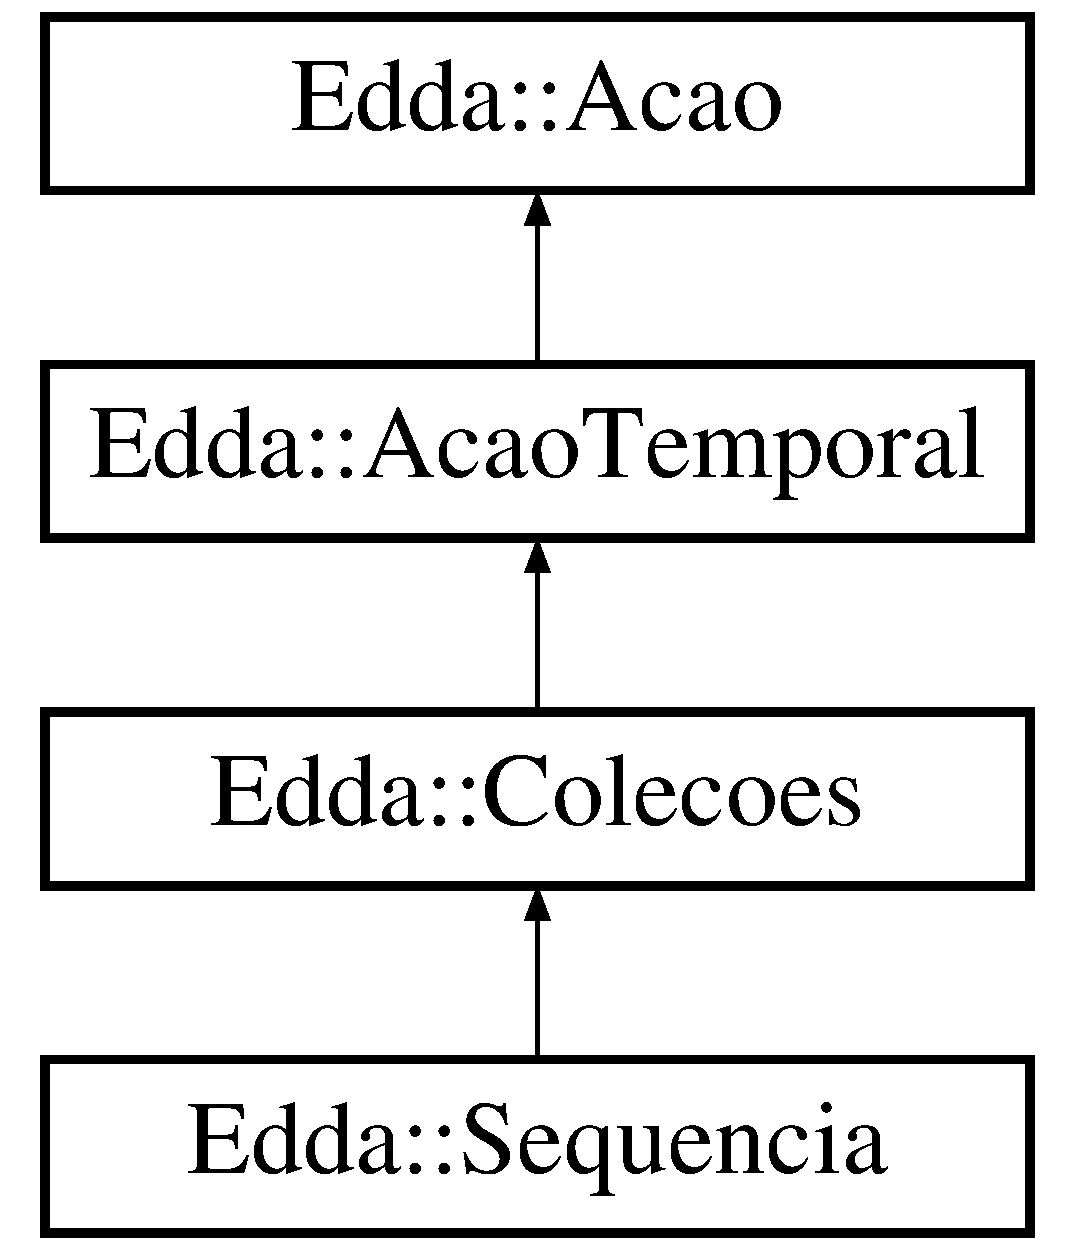
\includegraphics[height=4.000000cm]{class_edda_1_1_sequencia}
\end{center}
\end{figure}
\subsection*{Public Member Functions}
\begin{DoxyCompactItemize}
\item 
\hypertarget{class_edda_1_1_sequencia_a9b5257bbcd2d112c2b2b55fa69a23a34}{
void {\bfseries atualizar} (long)}
\label{class_edda_1_1_sequencia_a9b5257bbcd2d112c2b2b55fa69a23a34}

\end{DoxyCompactItemize}


The documentation for this class was generated from the following files:\begin{DoxyCompactItemize}
\item 
Sequencia.h\item 
Sequencia.cpp\end{DoxyCompactItemize}

\hypertarget{class_edda_1_1_sprite}{
\section{Edda::Sprite Class Reference}
\label{class_edda_1_1_sprite}\index{Edda::Sprite@{Edda::Sprite}}
}
Inheritance diagram for Edda::Sprite:\begin{figure}[H]
\begin{center}
\leavevmode
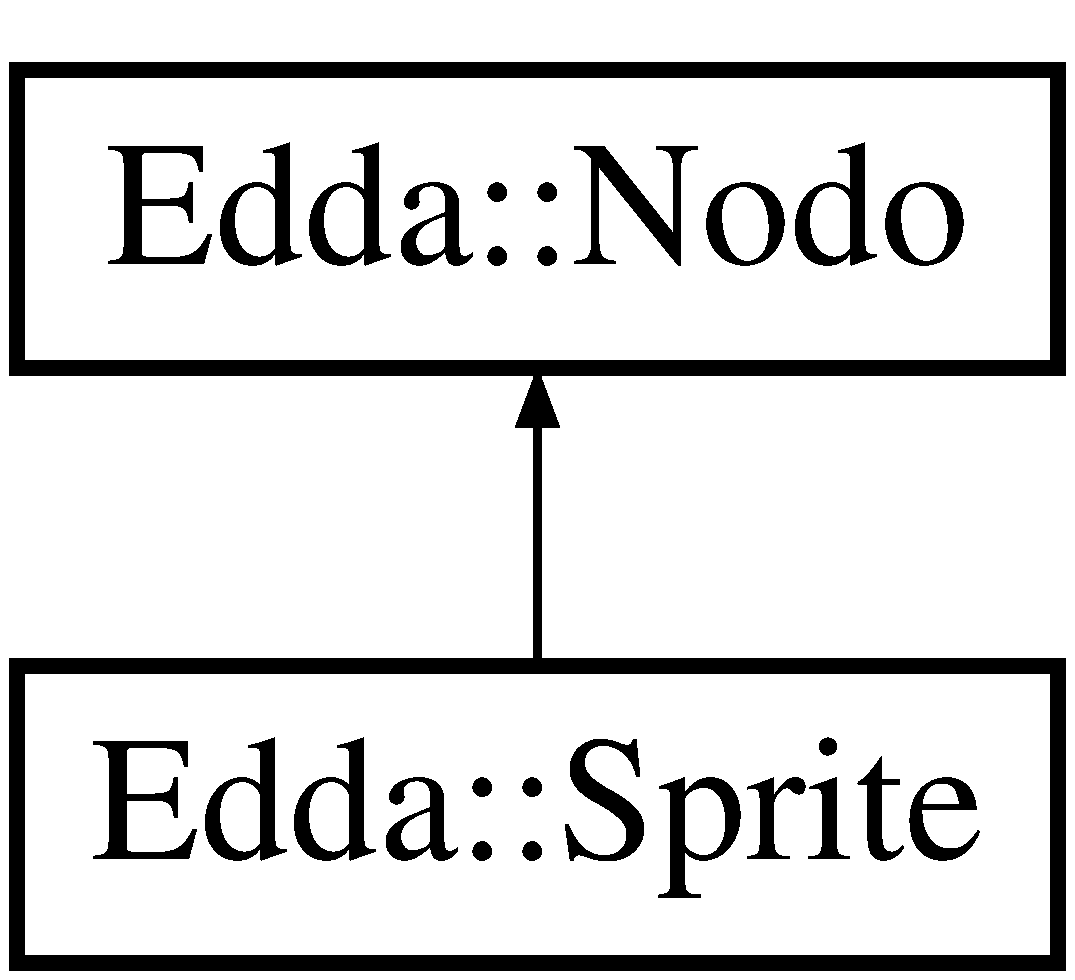
\includegraphics[height=2.000000cm]{class_edda_1_1_sprite}
\end{center}
\end{figure}
\subsection*{Public Member Functions}
\begin{DoxyCompactItemize}
\item 
\hypertarget{class_edda_1_1_sprite_af0f5a95c9e240ef31c3f7bd31e4a7b80}{
void {\bfseries carregarImagem} (string)}
\label{class_edda_1_1_sprite_af0f5a95c9e240ef31c3f7bd31e4a7b80}

\item 
\hypertarget{class_edda_1_1_sprite_a0c0c1248fd001977f2246d9d560a92a1}{
void {\bfseries carregarImagem} (string, int, int)}
\label{class_edda_1_1_sprite_a0c0c1248fd001977f2246d9d560a92a1}

\item 
\hypertarget{class_edda_1_1_sprite_a08c180e752e186a0130ac5413dca1909}{
void {\bfseries desenhar} (sf::RenderWindow $\ast$)}
\label{class_edda_1_1_sprite_a08c180e752e186a0130ac5413dca1909}

\item 
\hypertarget{class_edda_1_1_sprite_a67300b51eeeeacf197bceeafae0cc308}{
void {\bfseries setPosicao} (int, int)}
\label{class_edda_1_1_sprite_a67300b51eeeeacf197bceeafae0cc308}

\item 
\hypertarget{class_edda_1_1_sprite_a05dd1b485aca4b45e8685988a886d273}{
sf::Image $\ast$ {\bfseries getFrame} (int)}
\label{class_edda_1_1_sprite_a05dd1b485aca4b45e8685988a886d273}

\item 
\hypertarget{class_edda_1_1_sprite_a569770c988611814e3f712e80327f085}{
void {\bfseries setFrame} (int)}
\label{class_edda_1_1_sprite_a569770c988611814e3f712e80327f085}

\item 
\hypertarget{class_edda_1_1_sprite_aff9acd347a11e232857138d161547479}{
bool {\bfseries colidir} (\hyperlink{class_edda_1_1_sprite}{Sprite} $\ast$s, bool pixel=true)}
\label{class_edda_1_1_sprite_aff9acd347a11e232857138d161547479}

\item 
\hypertarget{class_edda_1_1_sprite_acebf844c4240554758e20327076a1ca9}{
void {\bfseries tratarEvento} (RenderWindow $\ast$)}
\label{class_edda_1_1_sprite_acebf844c4240554758e20327076a1ca9}

\end{DoxyCompactItemize}


The documentation for this class was generated from the following files:\begin{DoxyCompactItemize}
\item 
Sprite.h\item 
Sprite.cpp\end{DoxyCompactItemize}

\hypertarget{class_edda_1_1_tile}{
\section{Edda::Tile Class Reference}
\label{class_edda_1_1_tile}\index{Edda::Tile@{Edda::Tile}}
}
\subsection*{Public Member Functions}
\begin{DoxyCompactItemize}
\item 
\hypertarget{class_edda_1_1_tile_aa52aeaf8357fefd662f2bc770fb4e2e8}{
void {\bfseries setTile} (int num\_\-tile, int largura, int altura)}
\label{class_edda_1_1_tile_aa52aeaf8357fefd662f2bc770fb4e2e8}

\item 
\hypertarget{class_edda_1_1_tile_a8ce3dfb0c44ef4ff381580b34e5969ef}{
void {\bfseries setWalk} (bool bw)}
\label{class_edda_1_1_tile_a8ce3dfb0c44ef4ff381580b34e5969ef}

\item 
\hypertarget{class_edda_1_1_tile_a03da1dda6c1e5b2e5a79e9e0b04676f4}{
void {\bfseries setInfo} (int inf)}
\label{class_edda_1_1_tile_a03da1dda6c1e5b2e5a79e9e0b04676f4}

\item 
\hypertarget{class_edda_1_1_tile_a592e4c195d4aaf3fc2862c4830e043bc}{
int {\bfseries getInfo} ()}
\label{class_edda_1_1_tile_a592e4c195d4aaf3fc2862c4830e043bc}

\item 
\hypertarget{class_edda_1_1_tile_a7a2c8952aa1fd6260585ed4c63a4980a}{
bool {\bfseries getWalk} ()}
\label{class_edda_1_1_tile_a7a2c8952aa1fd6260585ed4c63a4980a}

\item 
\hypertarget{class_edda_1_1_tile_afbfdb5dbe3aae08926e1b1d8e6481d62}{
int {\bfseries getTileN} ()}
\label{class_edda_1_1_tile_afbfdb5dbe3aae08926e1b1d8e6481d62}

\item 
\hypertarget{class_edda_1_1_tile_ae8cb5b935bfa0f206c0eb9bf0d50fd28}{
int {\bfseries getX} ()}
\label{class_edda_1_1_tile_ae8cb5b935bfa0f206c0eb9bf0d50fd28}

\item 
\hypertarget{class_edda_1_1_tile_af455bc06ee873596b5b7848f1764ca48}{
int {\bfseries getY} ()}
\label{class_edda_1_1_tile_af455bc06ee873596b5b7848f1764ca48}

\end{DoxyCompactItemize}
\subsection*{Friends}
\begin{DoxyCompactItemize}
\item 
\hypertarget{class_edda_1_1_tile_abb3e8d219d526d16e351f7282f6a8bed}{
class {\bfseries Tilemap}}
\label{class_edda_1_1_tile_abb3e8d219d526d16e351f7282f6a8bed}

\end{DoxyCompactItemize}


The documentation for this class was generated from the following files:\begin{DoxyCompactItemize}
\item 
Tilemap.h\item 
Tile.cpp\end{DoxyCompactItemize}

\hypertarget{class_edda_1_1_tile_cache}{
\section{Edda::TileCache Class Reference}
\label{class_edda_1_1_tile_cache}\index{Edda::TileCache@{Edda::TileCache}}
}
\subsection*{Public Member Functions}
\begin{DoxyCompactItemize}
\item 
\hypertarget{class_edda_1_1_tile_cache_a6e4ce40b733c801d0e91003a772a0b1e}{
void {\bfseries desenhar} (RenderWindow $\ast$, int index, int x, int y)}
\label{class_edda_1_1_tile_cache_a6e4ce40b733c801d0e91003a772a0b1e}

\item 
\hypertarget{class_edda_1_1_tile_cache_afdb29418165b34a31acac9141e6ad86a}{
int {\bfseries carregar} (string arquivo)}
\label{class_edda_1_1_tile_cache_afdb29418165b34a31acac9141e6ad86a}

\item 
\hypertarget{class_edda_1_1_tile_cache_ab557295393831656906de2beae510097}{
int {\bfseries carregar} (string arquivo, int px, int py, int largura, int altura)}
\label{class_edda_1_1_tile_cache_ab557295393831656906de2beae510097}

\item 
\hypertarget{class_edda_1_1_tile_cache_a99411c6e969c40a74f11c1359e013005}{
int {\bfseries localizar} (string arquivo)}
\label{class_edda_1_1_tile_cache_a99411c6e969c40a74f11c1359e013005}

\item 
\hypertarget{class_edda_1_1_tile_cache_aa35a22d04966b02a1172e0c30d1785eb}{
\hyperlink{class_edda_1_1_sprite}{Sprite} $\ast$ {\bfseries getImagem} (int index)}
\label{class_edda_1_1_tile_cache_aa35a22d04966b02a1172e0c30d1785eb}

\item 
\hypertarget{class_edda_1_1_tile_cache_a3f86ee3d88a6718a0ba5e3768b8970d5}{
int {\bfseries getNumTiles} ()}
\label{class_edda_1_1_tile_cache_a3f86ee3d88a6718a0ba5e3768b8970d5}

\end{DoxyCompactItemize}
\subsection*{Static Public Member Functions}
\begin{DoxyCompactItemize}
\item 
\hypertarget{class_edda_1_1_tile_cache_a5863f2e38ab77273c33419bb5327f89d}{
static \hyperlink{class_edda_1_1_tile_cache}{TileCache} $\ast$ {\bfseries instance} ()}
\label{class_edda_1_1_tile_cache_a5863f2e38ab77273c33419bb5327f89d}

\item 
\hypertarget{class_edda_1_1_tile_cache_a7558ff2cd52db59d3c95517a0ab6a39c}{
static void {\bfseries destruir} ()}
\label{class_edda_1_1_tile_cache_a7558ff2cd52db59d3c95517a0ab6a39c}

\end{DoxyCompactItemize}


The documentation for this class was generated from the following files:\begin{DoxyCompactItemize}
\item 
Tilemap.h\item 
TileCache.cpp\end{DoxyCompactItemize}

\hypertarget{class_edda_1_1_tilemap}{
\section{Edda::Tilemap Class Reference}
\label{class_edda_1_1_tilemap}\index{Edda::Tilemap@{Edda::Tilemap}}
}
Inheritance diagram for Edda::Tilemap:\begin{figure}[H]
\begin{center}
\leavevmode
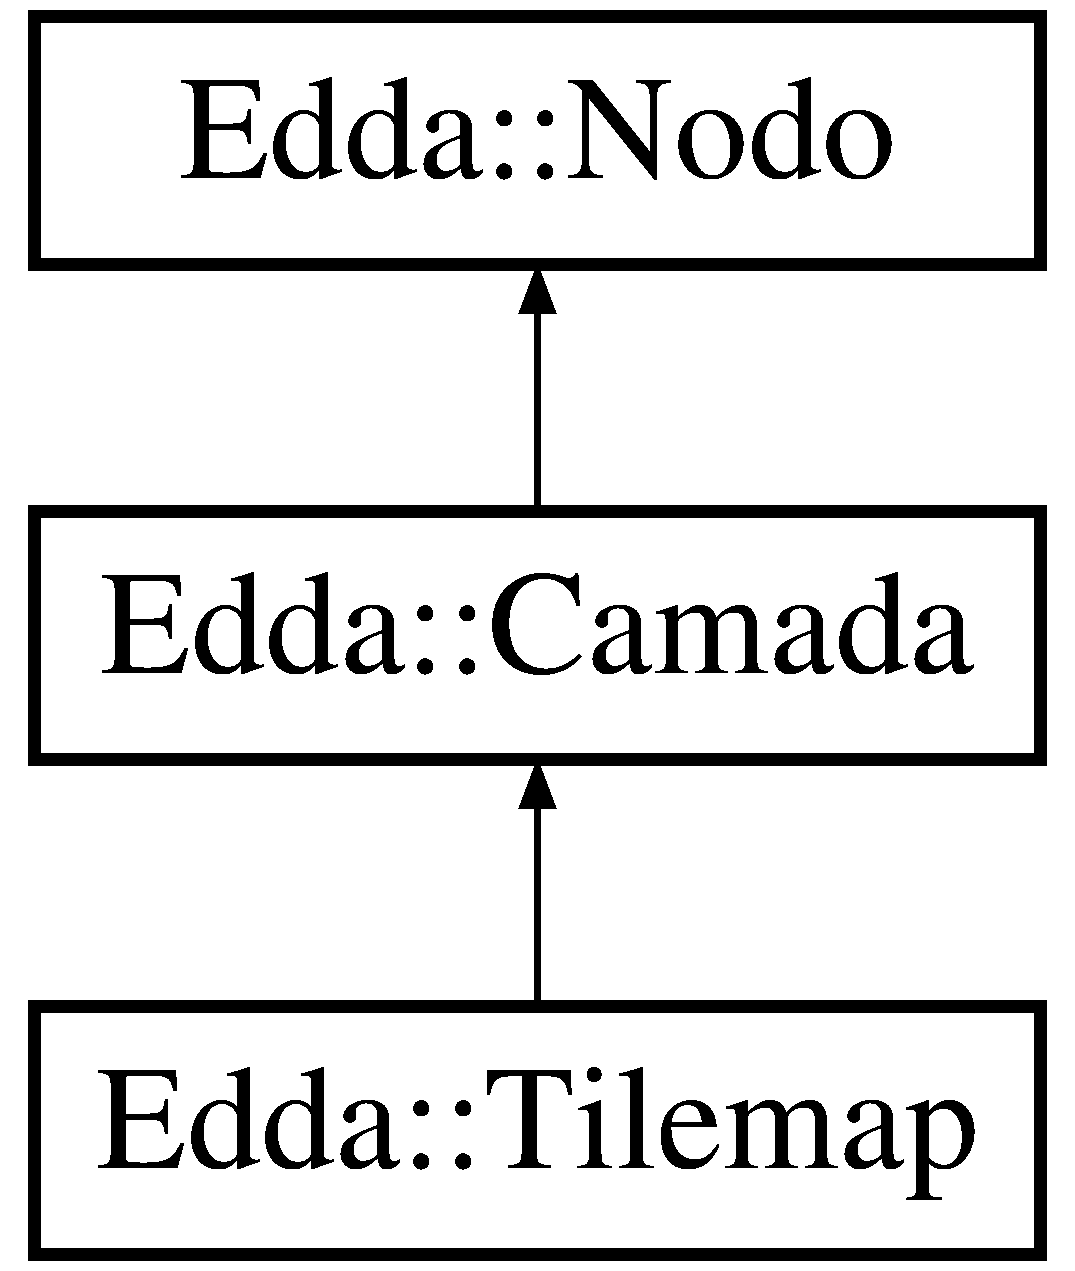
\includegraphics[height=3.000000cm]{class_edda_1_1_tilemap}
\end{center}
\end{figure}
\subsection*{Public Member Functions}
\begin{DoxyCompactItemize}
\item 
\hypertarget{class_edda_1_1_tilemap_a76524bc24f1ad9910410dec817ed3cbf}{
void {\bfseries desenhar} (RenderWindow $\ast$)}
\label{class_edda_1_1_tilemap_a76524bc24f1ad9910410dec817ed3cbf}

\item 
\hypertarget{class_edda_1_1_tilemap_a5acc405b96a2a9930a83e25f2bae739c}{
bool {\bfseries inicializa} (string arq)}
\label{class_edda_1_1_tilemap_a5acc405b96a2a9930a83e25f2bae739c}

\item 
\hypertarget{class_edda_1_1_tilemap_a05c8b0069bd66eeea1b9af9f04408063}{
void {\bfseries desenha} ()}
\label{class_edda_1_1_tilemap_a05c8b0069bd66eeea1b9af9f04408063}

\item 
\hypertarget{class_edda_1_1_tilemap_a84a6adb25af48e068ab107c5ac2be556}{
void {\bfseries move} (int dx, int dy)}
\label{class_edda_1_1_tilemap_a84a6adb25af48e068ab107c5ac2be556}

\item 
\hypertarget{class_edda_1_1_tilemap_a184b5c5a773673514f7a71556ae757a0}{
\hyperlink{class_edda_1_1_tile}{Tile} $\ast$ {\bfseries getTile} (int \_\-x, int \_\-y)}
\label{class_edda_1_1_tilemap_a184b5c5a773673514f7a71556ae757a0}

\item 
\hypertarget{class_edda_1_1_tilemap_a137da551ada18de39eed323b3ec17363}{
void {\bfseries screen2map} (int x, int y, int \&mx, int \&my)}
\label{class_edda_1_1_tilemap_a137da551ada18de39eed323b3ec17363}

\item 
\hypertarget{class_edda_1_1_tilemap_adcfe41aafcd25aef74d3caa29f1faf5b}{
void {\bfseries map2screen} (int x, int y, int \&mx, int \&my)}
\label{class_edda_1_1_tilemap_adcfe41aafcd25aef74d3caa29f1faf5b}

\item 
\hypertarget{class_edda_1_1_tilemap_a5e8ca0394395e9f9edf0406ffc8301b6}{
int {\bfseries XparaTela} (int mx)}
\label{class_edda_1_1_tilemap_a5e8ca0394395e9f9edf0406ffc8301b6}

\item 
\hypertarget{class_edda_1_1_tilemap_a5844165095af2ef3c19e812cb65f43c7}{
int {\bfseries YparaTela} (int my)}
\label{class_edda_1_1_tilemap_a5844165095af2ef3c19e812cb65f43c7}

\item 
\hypertarget{class_edda_1_1_tilemap_a266f422a080bd77925db78c67298e1c8}{
bool {\bfseries pointColTile} (int x, int y, int \&cx, int \&cy)}
\label{class_edda_1_1_tilemap_a266f422a080bd77925db78c67298e1c8}

\item 
\hypertarget{class_edda_1_1_tilemap_a505e0156b76397fb948bac0062be0f7b}{
bool {\bfseries colide} (int x, int y, int w, int h)}
\label{class_edda_1_1_tilemap_a505e0156b76397fb948bac0062be0f7b}

\item 
\hypertarget{class_edda_1_1_tilemap_a56abd23dedcb11aa634a33502faf7e02}{
int {\bfseries getTileW} ()}
\label{class_edda_1_1_tilemap_a56abd23dedcb11aa634a33502faf7e02}

\item 
\hypertarget{class_edda_1_1_tilemap_a9d2e45237be01d8a42eb73bde7f5e040}{
int {\bfseries getTileH} ()}
\label{class_edda_1_1_tilemap_a9d2e45237be01d8a42eb73bde7f5e040}

\end{DoxyCompactItemize}


The documentation for this class was generated from the following files:\begin{DoxyCompactItemize}
\item 
Tilemap.h\item 
Tilemap.cpp\end{DoxyCompactItemize}

\printindex
\end{document}
